\title{三角函数（2016--2025 高考真题）}
\author{}
\date{}
\maketitle
\noindent 本专题共 111 道题，按年份排列。每题标注原卷与原题号。

\section*{2016 年}

\begin{question}[points=5]
\textbf{来源：}2016 年 全国III卷-理科，第 5 题\par
若 $\tan\alpha=\frac{3}{4}$, 则 $\cos^2\alpha+2\sin2\alpha=$
\begin{choices}
  \item $\frac{64}{25}$
  \item $\frac{48}{25}$
  \item $1$
  \item $\frac{16}{25}$
\end{choices}
\begin{solution}
\textbf{答案：}$\frac{64}{25}$

\textbf{分析：}将所求的关系式的分母 "$1$" 化为 $(\cos^2\alpha+\sin^2\alpha)$, 再将 "弦" 化 "切" 即可得到答案.

\textbf{详解：}$\because\tan\alpha=\frac{3}{4}$, $\therefore\cos^2\alpha+2\sin2\alpha=\frac{\cos^2\alpha+4\sin\alpha\cos\alpha}{\cos^2\alpha+\sin^2\alpha}=\frac{1+4\tan\alpha}{1+\tan^2\alpha}=\frac{1+3}{1+\frac{9}{16}}=\frac{4}{\frac{25}{16}}=\frac{64}{25}$, 故选 A.
\end{solution}
\end{question}

\begin{question}[points=5]
\textbf{来源：}2016 年 全国III卷-理科，第 14 题\par
函数 $y=\sin x-\sqrt{3}\cos x$ 的图象可由函数 $y=\sin x+\sqrt{3}\cos x$ 的图象至少向右平移  个单位长度得到.
\fillin[{$\frac{2\pi}{3}$}]
\begin{solution}
\textbf{答案：}$\frac{2\pi}{3}$

\textbf{分析：}令 $f(x)=\sin x+\sqrt{3}\cos x=2\sin(x+\frac{\pi}{3})$, 则 $f(x-\phi)=2\sin(x+\frac{\pi}{3}-\phi)$, 依题意可得 $2\sin(x+\frac{\pi}{3}-\phi)=2\sin(x-\frac{\pi}{3})$, 由 $\frac{\pi}{3}-\phi=2k\pi-\frac{\pi}{3}$ 可得答案.

\textbf{详解：}$y=f(x)=\sin x+\sqrt{3}\cos x=2\sin(x+\frac{\pi}{3})$, $y=\sin x-\sqrt{3}\cos x=2\sin(x-\frac{\pi}{3})$. $f(x-\phi)=2\sin(x+\frac{\pi}{3}-\phi)$ ($\phi>0$), 令 $2\sin(x+\frac{\pi}{3}-\phi)=2\sin(x-\frac{\pi}{3})$, 则 $\frac{\pi}{3}-\phi=2k\pi-\frac{\pi}{3}$, 即 $\phi=\frac{2\pi}{3}-2k\pi$, 当 $k=0$ 时, 正数 $\phi_{\min}=\frac{2\pi}{3}$. 故答案为 $\frac{2\pi}{3}$.
\end{solution}
\end{question}

\begin{question}[points=12]
\textbf{来源：}2016 年 全国III卷-理科，第 21 题；次专题：导数\par
设函数 $f(x)=a\cos2x+(a-1)(\cos x+1)$, 其中 $a>0$, 记 $|f(x)|$ 的最大值为 $A$.

(Ⅰ) 求 $f'(x)$;

(Ⅱ) 求 $A$;

(Ⅲ) 证明: $|f'(x)|\le2A$.
\begin{solution}

\textbf{分析：}(Ⅰ) 根据复合函数的导数公式进行求解. (Ⅱ) 讨论 $a$ 的取值, 利用分类讨论的思想方法, 结合换元法以及一元二次函数的最值的性质进行求解. (Ⅲ) 结合绝对值不等式的性质即可证明.

\textbf{详解：}(Ⅰ) 解: $f'(x)=-2a\sin2x-(a-1)\sin x$.
(Ⅱ) 当 $a\ge1$ 时, $|f(x)|=|a\cos2x+(a-1)(\cos x+1)|\le a|\cos2x|+(a-1)|\cos x+1|\le a|\cos2x|+(a-1)(|\cos x|+1)\le a+2(a-1)=3a-2=f(0)$, 因此 $A=3a-2$. 当 $0<a<1$ 时, $f(x)=a\cos2x+(a-1)(\cos x+1)=2a\cos^2x+(a-1)\cos x-1$, 令 $g(t)=2at^2+(a-1)t-1$, 则 $A$ 是 $|g(t)|$ 在 $[-1,1]$ 上的最大值, $g(-1)=a$, $g(1)=3a-2$, 且当 $t=\frac{1-a}{4a}$ 时, $g(t)$ 取得极小值 $g(\frac{1-a}{4a})=-\frac{(a-1)^2}{8a}-1=-\frac{(a-1)^2+8a}{8a}=-\frac{a^2+6a+1}{8a}$. 令 $-1<\frac{1-a}{4a}<1$, 得 $a>\frac{1}{5}$. ①当 $0<a\le\frac{1}{5}$ 时, $g(t)$ 在 $(-1,1)$ 内无极值点, $|g(-1)|=a$, $|g(1)|=2-3a$, $|g(-1)|<|g(1)|$, $\therefore A=2-3a$; ②当 $\frac{1}{5}<a<1$ 时, 由 $g(-1)-g(1)=2(1-a)>0$, 得 $g(-1)>g(1)>g(\frac{1-a}{4a})$, 又 $|g(\frac{1-a}{4a})|-|g(-1)|=\frac{(1-a)^2}{8a}-\frac{(1-a)^2}{8a}?$ 实际上 $|g(\frac{1-a}{4a})|=\frac{a^2+6a+1}{8a}$, $|g(-1)|=a$, $\frac{a^2+6a+1}{8a}-a=\frac{a^2+6a+1-8a^2}{8a}=\frac{-7a^2+6a+1}{8a}=\frac{-(7a+1)(a-1)}{8a}>0$, $\therefore A=|g(\frac{1-a}{4a})|=\frac{a^2+6a+1}{8a}$. 综上, $A=\begin{cases}2-3a, &0<a\le\frac{1}{5}\\ \frac{a^2+6a+1}{8a}, &\frac{1}{5}<a<1\\ 3a-2, &a\ge1\end{cases}$.
(Ⅲ) 证明: 由(Ⅰ)可得 $|f'(x)|=|-2a\sin2x-(a-1)\sin x|\le2a+|a-1|$. 当 $0<a\le\frac{1}{5}$ 时, $|f'(x)|<1+a\le2-4a<2(2-3a)=2A$; 当 $\frac{1}{5}<a<1$ 时, $A=\frac{a^2+6a+1}{8a}=\frac{a}{8}+\frac{3}{4}+\frac{1}{8a}>1$, $\therefore|f'(x)|\le1+a\le2A$; 当 $a\ge1$ 时, $|f'(x)|\le3a-1\le6a-4=2A$. 综上, $|f'(x)|\le2A$.
\end{solution}
\end{question}

\begin{question}[points=5]
\textbf{来源：}2016 年 全国III卷-文科，第 6 题\par
若 $\tan\theta=\dfrac{1}{3}$, 则 $\cos2\theta=$ ( )
\begin{choices}
  \item $\dfrac{4}{5}$
  \item $\dfrac{1}{5}$
  \item $\dfrac{1}{5}$
  \item $\dfrac{3}{5}$
\end{choices}
\begin{solution}
\textbf{答案：}$\dfrac{4}{5}$

\textbf{分析：}原式利用二倍角的余弦函数公式变形, 再利用同角三角函数间的基本关系化简, 将 $\tan\theta$ 的值代入计算即可求出值.

\textbf{详解：}$\tan\theta=\dfrac{1}{3}$, 则 $\cos2\theta=2\cos^2\theta-1=\dfrac{2}{1+\tan^2\theta}-1=\dfrac{2}{1+\frac{1}{9}}-1=\dfrac{2}{\frac{10}{9}}-1=\dfrac{18}{10}-1=\dfrac{8}{10}=\dfrac{4}{5}$. 故选 D.
\end{solution}
\end{question}

\begin{question}[points=5]
\textbf{来源：}2016 年 全国III卷-文科，第 14 题\par
函数 $y=\sin x-\sqrt{3}\cos x$ 的图象可由函数 $y=2\sin x$ 的图象至少向右平移  个单位长度得到.
\fillin[{$\dfrac{\pi}{3}$}]
\begin{solution}
\textbf{答案：}$\dfrac{\pi}{3}$

\textbf{分析：}令 $f(x)=2\sin x$, 则 $f(x-\varphi)=2\sin(x-\varphi)$, 依题意可得 $2\sin(x-\varphi)=2\sin(x-\frac{\pi}{3})$, 由 $-\varphi=2k\pi-\frac{\pi}{3}$ $(k\in\mathbb{Z})$, 可得答案.

\textbf{详解：}$y=\sin x-\sqrt{3}\cos x=2\sin(x-\frac{\pi}{3})$. 令 $f(x)=2\sin x$, 则 $f(x-\varphi)=2\sin(x-\varphi)$ $(\varphi>0)$. 依题意 $2\sin(x-\varphi)=2\sin(x-\frac{\pi}{3})$, 故 $-\varphi=2k\pi-\frac{\pi}{3}$ $(k\in\mathbb{Z})$, 即 $\varphi=-2k\pi+\frac{\pi}{3}$ $(k\in\mathbb{Z})$. 当 $k=0$ 时, 正数 $\varphi_{\min}=\dfrac{\pi}{3}$. 故答案为 $\dfrac{\pi}{3}$.
\end{solution}
\end{question}

\begin{question}[points=5]
\textbf{来源：}2016 年 全国II卷-理科，第 7 题\par
若将函数$y=2\sin2x$的图象向左平移$\frac{\pi}{12}$个单位长度，则平移后的图象的对称轴为（\quad）
\begin{choices}
  \item $x=\frac{k\pi}{2}-\frac{\pi}{6}\ (k\in\mathbb{Z})$
  \item $x=\frac{k\pi}{2}+\frac{\pi}{6}\ (k\in\mathbb{Z})$
  \item $x=\frac{k\pi}{2}-\frac{\pi}{12}\ (k\in\mathbb{Z})$
  \item $x=\frac{k\pi}{2}+\frac{\pi}{12}\ (k\in\mathbb{Z})$
\end{choices}
\begin{solution}
\textbf{答案：}$x=\frac{k\pi}{2}+\frac{\pi}{6}\ (k\in\mathbb{Z})$

\textbf{分析：}利用函数$y=A\sin(\omega x+\varphi)$的图象的变换及正弦函数的对称性可得答案．

\textbf{详解：}平移后得$y=2\sin\left[2\left(x+\frac{\pi}{12}\right)\right]=2\sin\left(2x+\frac{\pi}{6}\right)$，令$2x+\frac{\pi}{6}=k\pi+\frac{\pi}{2}$，得$x=\frac{k\pi}{2}+\frac{\pi}{6}$．故选B．
\end{solution}
\end{question}

\begin{question}[points=5]
\textbf{来源：}2016 年 全国II卷-理科，第 9 题\par
若$\cos\left(\frac{\pi}{4}-\alpha\right)=\frac{3}{5}$，则$\sin2\alpha=$（\quad）
\begin{choices}
  \item $\frac{7}{25}$
  \item $\frac{1}{5}$
  \item $-\frac{1}{5}$
  \item $-\frac{7}{25}$
\end{choices}
\begin{solution}
\textbf{答案：}$-\frac{7}{25}$

\textbf{分析：}法1：利用诱导公式化$\sin2\alpha=\cos\left(\frac{\pi}{2}-2\alpha\right)$，再利用二倍角的余弦可得答案．法2：利用余弦二倍角公式将左边展开，可以得$\sin\alpha+\cos\alpha$的值，再平方，即得$\sin2\alpha$的值．

\textbf{详解：}法1：$\sin2\alpha=\cos\left(\frac{\pi}{2}-2\alpha\right)=\cos\left[2\left(\frac{\pi}{4}-\alpha\right)\right]=2\cos^2\left(\frac{\pi}{4}-\alpha\right)-1=2\times\frac{9}{25}-1=-\frac{7}{25}$．故选D．
\end{solution}
\end{question}

\begin{question}[points=5]
\textbf{来源：}2016 年 全国II卷-文科，第 3 题\par
函数$y=A\sin(\omega x+\varphi)$的部分图象如图所示，则

\begin{center}
  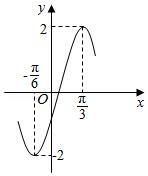
\includegraphics[width=.42\linewidth]{assets/asset-008-01.jpg}
\end{center}
\begin{choices}
  \item $y=2\sin(2x-\frac{\pi}{6})$
  \item $y=2\sin(2x-\frac{\pi}{3})$
  \item $y=2\sin(x+\frac{\pi}{6})$
  \item $y=2\sin(x+\frac{\pi}{3})$
\end{choices}
\begin{solution}
\textbf{答案：}$y=2\sin(2x-\frac{\pi}{6})$

\textbf{分析：}由图得$A=2$，$\frac{T}{4}=\frac{\pi}{4}$，故$T=\pi$，$\omega=2$，代入点$(\frac{\pi}{12},2)$得$\varphi=-\frac{\pi}{6}$。
\end{solution}
\end{question}

\begin{question}[points=5]
\textbf{来源：}2016 年 全国II卷-文科，第 11 题\par
函数$f(x)=\cos2x+6\cos(\frac{\pi}{2}-x)$的最大值为
\begin{choices}
  \item $4$
  \item $5$
  \item $6$
  \item $7$
\end{choices}
\begin{solution}
\textbf{答案：}$5$

\textbf{分析：}$f(x)=1-2\sin^2x+6\sin x$，令$t=\sin x\in[-1,1]$，$y=-2t^2+6t+1$，对称轴$t=\frac{3}{2}\notin[-1,1]$，在$[-1,1]$递增，$t=1$时$y_{\max}=5$。
\end{solution}
\end{question}

\begin{question}[points=5]
\textbf{来源：}2016 年 全国I卷-理科，第 12 题\par
已知函数$f(x)=\sin(\omega x+\varphi)$（$\omega>0$，$|\varphi|\le\frac{\pi}{2}$），$x=-\frac{\pi}{4}$为$f(x)$的零点，$x=\frac{\pi}{4}$为$y=f(x)$图象的对称轴，且$f(x)$在$(\frac{\pi}{18},\frac{5\pi}{36})$上单调，则$\omega$的最大值为（ ）
\begin{choices}
  \item $11$
  \item $9$
  \item $7$
  \item $5$
\end{choices}
\begin{solution}
\textbf{答案：}B

\textbf{分析：}根据已知可得$\omega$为正奇数，且$\omega\le12$，结合$x=-\frac{\pi}{4}$为$f(x)$的零点，$x=\frac{\pi}{4}$为$y=f(x)$图象的对称轴，求出满足条件的解析式，并结合$f(x)$在$(\frac{\pi}{18},\frac{5\pi}{36})$上单调，可得$\omega$的最大值．

\textbf{详解：}解：因为$x=-\frac{\pi}{4}$为$f(x)$的零点，$x=\frac{\pi}{4}$为$y=f(x)$图象的对称轴，所以$\frac{\pi}{4}-(-\frac{\pi}{4})=\frac{\pi}{2}=\frac{T}{4}+\frac{kT}{2}$，即$\frac{\pi}{2}=\frac{2\pi}{\omega}(\frac{1}{4}+\frac{k}{2})$，$\omega=2n+1$，$n\in N$即$\omega$为正奇数，因为$f(x)$在$(\frac{\pi}{18},\frac{5\pi}{36})$上单调，则$\frac{5\pi}{36}-\frac{\pi}{18}=\frac{\pi}{12}\le\frac{T}{2}$，即$T=\frac{2\pi}{\omega}\ge\frac{\pi}{6}$，解得：$\omega\le12$，当$\omega=11$时，$-\frac{11\pi}{4}+\varphi=k\pi$，$k\in Z$，因为$|\varphi|\le\frac{\pi}{2}$，所以$\varphi=-\frac{\pi}{4}$，此时$f(x)$在$(\frac{\pi}{18},\frac{5\pi}{36})$不单调，不满足题意；当$\omega=9$时，$-\frac{9\pi}{4}+\varphi=k\pi$，$k\in Z$，因为$|\varphi|\le\frac{\pi}{2}$，所以$\varphi=\frac{\pi}{4}$，此时$f(x)$在$(\frac{\pi}{18},\frac{5\pi}{36})$单调，满足题意；故$\omega$的最大值为$9$，故选：$B$．
\end{solution}
\end{question}

\begin{question}[points=5]
\textbf{来源：}2016 年 全国I卷-文科，第 6 题\par
将函数$y=2\sin(2x+\frac{\pi}{6})$的图象向右平移$\frac{1}{4}$个周期后，所得图象对应的函数为
\begin{choices}
  \item $y=2\sin(2x+\frac{\pi}{4})$
  \item $y=2\sin(2x+\frac{\pi}{3})$
  \item $y=2\sin(2x-\frac{\pi}{4})$
  \item $y=2\sin(2x-\frac{\pi}{3})$
\end{choices}
\begin{solution}
\textbf{答案：}$y=2\sin(2x-\frac{\pi}{3})$

\textbf{分析：}求得函数$y$的最小正周期，即有所对的函数式为$y=2\sin[2(x-\frac{\pi}{4})+\frac{\pi}{6}]$，化简整理即可得到所求函数式。

\textbf{详解：}函数$y=2\sin(2x+\frac{\pi}{6})$的周期为$T=\frac{2\pi}{2}=\pi$，由题意即为函数$y=2\sin(2x+\frac{\pi}{6})$的图象向右平移$\frac{\pi}{4}$个单位，可得图象对应的函数为$y=2\sin[2(x-\frac{\pi}{4})+\frac{\pi}{6}]$，即有$y=2\sin(2x-\frac{\pi}{3})$。故选：$D$。
\end{solution}
\end{question}

\begin{question}[points=5]
\textbf{来源：}2016 年 全国I卷-文科，第 14 题\par
已知$\theta$是第四象限角，且$\sin(\theta+\frac{\pi}{4})=\frac{3}{5}$，则$\tan(\theta-\frac{\pi}{4})=$
\fillin[{$-\frac{4}{3}$}]
\begin{solution}
\textbf{答案：}$-\frac{4}{3}$

\textbf{分析：}由$\theta$得范围求得$\theta+\frac{\pi}{4}$的范围，结合已知求得$\cos(\theta+\frac{\pi}{4})$，再由诱导公式求得$\sin(\frac{\pi}{4}-\theta)$及$\cos(\frac{\pi}{4}-\theta)$，进一步由诱导公式及同角三角函数基本关系式求得$\tan(\theta-\frac{\pi}{4})$的值。

\textbf{详解：}$\because\theta$是第四象限角，$\therefore -\frac{\pi}{2}+2k\pi<\theta<2k\pi$，则$-\frac{\pi}{4}+2k\pi<\theta+\frac{\pi}{4}<\frac{\pi}{4}+2k\pi$，又$\sin(\theta+\frac{\pi}{4})=\frac{3}{5}$，$\therefore\cos(\theta+\frac{\pi}{4})=\frac{4}{5}$。$\therefore\cos(\frac{\pi}{4}-\theta)=\sin(\theta+\frac{\pi}{4})=\frac{3}{5}$，$\sin(\frac{\pi}{4}-\theta)=\cos(\theta+\frac{\pi}{4})=\frac{4}{5}$。则$\tan(\theta-\frac{\pi}{4})=-\tan(\frac{\pi}{4}-\theta)=-\frac{\sin(\frac{\pi}{4}-\theta)}{\cos(\frac{\pi}{4}-\theta)}=-\frac{4}{3}$。故答案为：$-\frac{4}{3}$。
\end{solution}
\end{question}

\section*{2017 年}

\begin{question}[points=5]
\textbf{来源：}2017 年 全国III卷-理科，第 6 题\par
设函数$f(x)=\cos(x+\frac{\pi}{3})$，则下列结论错误的是（ ）
\begin{choices}
  \item $A$．$f(x)$的一个周期为$-2\pi$
  \item $B$．$y=f(x)$的图象关于直线$x=\frac{8\pi}{3}$对称
  \item $C$．$f(x+\pi)$的一个零点为$x=\frac{\pi}{6}$
  \item $D$．$f(x)$在$(\frac{\pi}{2},\pi)$单调递减
\end{choices}
\begin{solution}
\textbf{答案：}$D$

\textbf{分析：}根据三角函数的图象和性质分别进行判断即可。

\textbf{详解：}A．函数的周期为$2k\pi$，当$k=-1$时，周期$T=-2\pi$，故A正确。B．当$x=\frac{8\pi}{3}$时，$\cos(\frac{8\pi}{3}+\frac{\pi}{3})=\cos(3\pi)=-1$为最小值，此时$y=f(x)$的图象关于直线$x=\frac{8\pi}{3}$对称，故B正确。C．当$x=\frac{\pi}{6}$时，$f(\frac{\pi}{6}+\pi)=\cos(\frac{\pi}{6}+\pi+\frac{\pi}{3})=\cos\frac{3\pi}{2}=0$，则$f(x+\pi)$的一个零点为$x=\frac{\pi}{6}$，故C正确。D．当$\frac{\pi}{2}<x<\pi$时，$\frac{5\pi}{6}<x+\frac{\pi}{3}<\frac{4\pi}{3}$，此时函数$f(x)$不是单调函数，故D错误。故选D。
\end{solution}
\end{question}

\begin{question}[points=5]
\textbf{来源：}2017 年 全国III卷-文科，第 4 题\par
已知$\sin\alpha-\cos\alpha=\frac{4}{3}$，则$\sin2\alpha=$（    ）
\begin{choices}
  \item A．$-\frac{7}{9}$
  \item B．$-\frac{2}{9}$
  \item C．$\frac{2}{9}$
  \item D．$\frac{7}{9}$
\end{choices}
\begin{solution}
\textbf{答案：}A

\textbf{分析：}由条件，两边平方，根据二倍角公式和平方关系即可求出。

\textbf{详解：}由$\sin\alpha-\cos\alpha=\frac{4}{3}$，平方得$1-\sin2\alpha=\frac{16}{9}$，所以$\sin2\alpha=-\frac{7}{9}$。
\end{solution}
\end{question}

\begin{question}[points=5]
\textbf{来源：}2017 年 全国III卷-文科，第 6 题\par
函数$f(x)=\frac{1}{5}\sin(x+\frac{\pi}{3})+\cos(x-\frac{\pi}{6})$的最大值为（   ）
\begin{choices}
  \item A．$\frac{6}{5}$
  \item B．$1$
  \item C．$\frac{3}{5}$
  \item D．$\frac{1}{5}$
\end{choices}
\begin{solution}
\textbf{答案：}A

\textbf{分析：}利用诱导公式化简函数的解析式，通过正弦函数的最值求解即可。

\textbf{详解：}$f(x)=\frac{1}{5}\sin(x+\frac{\pi}{3})+\cos(x-\frac{\pi}{6})=\frac{1}{5}\sin(x+\frac{\pi}{3})+\sin(x+\frac{\pi}{3})=\frac{6}{5}\sin(x+\frac{\pi}{3})$，最大值为$\frac{6}{5}$。
\end{solution}
\end{question}

\begin{question}[points=5]
\textbf{来源：}2017 年 全国II卷-理科，第 14 题\par
函数 $f(x)=\sin^2x+\sqrt{3}\cos x-\frac{3}{4}$（$x\in[0,\frac{\pi}{2}]$）的最大值是 ．
\fillin[{$1$}]
\begin{solution}
\textbf{答案：}$1$

\textbf{分析：}同角的三角函数的关系以及二次函数的性质即可求出。

\textbf{详解：}$f(x)=\sin^2x+\sqrt{3}\cos x-\frac{3}{4}=1-\cos^2x+\sqrt{3}\cos x-\frac{3}{4}$，令 $\cos x=t$ 且 $t\in[0,1]$，则 $y=-t^2+\sqrt{3}t+\frac{1}{4}=-(t-\frac{\sqrt{3}}{2})^2+1$，当 $t=\frac{\sqrt{3}}{2}$ 时，$f(t)_{\max}=1$，即 $f(x)$ 的最大值为 $1$，故答案为：$1$。
\end{solution}
\end{question}

\begin{question}[points=5]
\textbf{来源：}2017 年 全国II卷-文科，第 3 题\par
函数 $f(x)=\sin\left(2x+\frac{\pi}{3}\right)$ 的最小正周期为
\begin{choices}
  \item $4\pi$
  \item $2\pi$
  \item $\pi$
  \item $\frac{\pi}{2}$
\end{choices}
\begin{solution}
\textbf{答案：}$\pi$

\textbf{分析：}利用三角函数周期公式, 直接求解即可.

\textbf{详解：}函数 $f(x)=\sin\left(2x+\frac{\pi}{3}\right)$ 的最小正周期为 $\frac{2\pi}{2}=\pi$. 故选C.
\end{solution}
\end{question}

\begin{question}[points=5]
\textbf{来源：}2017 年 全国II卷-文科，第 13 题\par
函数 $f(x)=2\cos x+\sin x$ 的最大值为
\fillin[{$\sqrt{5}$}]
\begin{solution}
\textbf{答案：}$\sqrt{5}$

\textbf{分析：}利用辅助角公式化简函数的解析式, 通过正弦函数的有界性求解即可.

\textbf{详解：}函数 $f(x)=2\cos x+\sin x=\sqrt{5}\left(\frac{2}{\sqrt{5}}\cos x+\frac{1}{\sqrt{5}}\sin x\right)=\sqrt{5}\sin(x+\theta)$, 其中 $\tan\theta=2$, 可知函数的最大值为 $\sqrt{5}$. 故答案为 $\sqrt{5}$.
\end{solution}
\end{question}

\begin{question}[points=5]
\textbf{来源：}2017 年 全国I卷-理科，第 9 题\par
已知曲线 $C_1:y=\cos x$，$C_2:y=\sin\left(2x+\frac{2\pi}{3}\right)$，则下面结论正确的是（ ）
\begin{choices}
  \item 把 $C_1$ 上各点的横坐标伸长到原来的 2 倍，纵坐标不变，再把得到的曲线向右平移 $\frac{\pi}{6}$ 个单位长度，得到曲线 $C_2$
  \item 把 $C_1$ 上各点的横坐标伸长到原来的 2 倍，纵坐标不变，再把得到的曲线向左平移 $\frac{\pi}{12}$ 个单位长度，得到曲线 $C_2$
  \item 把 $C_1$ 上各点的横坐标缩短到原来的 $\frac{1}{2}$ 倍，纵坐标不变，再把得到的曲线向右平移 $\frac{\pi}{6}$ 个单位长度，得到曲线 $C_2$
  \item 把 $C_1$ 上各点的横坐标缩短到原来的 $\frac{1}{2}$ 倍，纵坐标不变，再把得到的曲线向左平移 $\frac{\pi}{12}$ 个单位长度，得到曲线 $C_2$
\end{choices}
\begin{solution}
\textbf{答案：}D

\textbf{分析：}利用三角函数的伸缩变换以及平移变换转化求解即可．

\textbf{详解：}把 $C_1$ 上各点的横坐标缩短到原来的 $\frac{1}{2}$ 倍，纵坐标不变，得到函数 $y=\cos 2x$ 图象，再把得到的曲线向左平移 $\frac{\pi}{12}$ 个单位长度，得到函数 $y=\cos\left[2\left(x+\frac{\pi}{12}\right)\right]=\cos\left(2x+\frac{\pi}{6}\right)=\sin\left(2x+\frac{2\pi}{3}\right)$ 的图象，即曲线 $C_2$．故选：D．
\end{solution}
\end{question}

\begin{question}[points=5]
\textbf{来源：}2017 年 全国I卷-文科，第 8 题\par
函数$y=\frac{\sin x}{1+\cos x}$的部分图象大致为（        ）

\begin{center}
  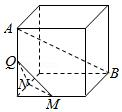
\includegraphics[width=.42\linewidth]{assets/asset-020-01.jpg}
\end{center}
\begin{choices}
  \item 
  \item 
  \item 
  \item 
\end{choices}
\begin{solution}
\textbf{答案：}C

\textbf{分析：}判断函数的奇偶性排除选项，利用特殊值判断即可。

\textbf{详解：}解：函数$y=\frac{\sin x}{1+\cos x}$，可知函数是奇函数，排除选项B，当$x=\frac{\pi}{2}$时，$f(\frac{\pi}{2})=\frac{1}{1+0}=1$，排除A，$x=\pi$时，$f(\pi)=0$，排除D。故选：C。
\end{solution}
\end{question}

\begin{question}[points=5]
\textbf{来源：}2017 年 全国I卷-文科，第 15 题\par
已知$\alpha\in(0,\frac{\pi}{2})$，$\tan\alpha=2$，则$\cos(\alpha-\frac{\pi}{4})=$ ．
\fillin[{$\frac{3\sqrt{10}}{10}$}]
\begin{solution}
\textbf{答案：}$\frac{3\sqrt{10}}{10}$

\textbf{分析：}根据同角的三角函数的关系求出$\sin\alpha=\frac{2\sqrt{5}}{5}$，$\cos\alpha=\frac{\sqrt{5}}{5}$，再根据两角差的余弦公式即可求出。

\textbf{详解：}解：$\because\alpha\in(0,\frac{\pi}{2})$，$\tan\alpha=2$，$\therefore\sin\alpha=2\cos\alpha$，$\because\sin^2\alpha+\cos^2\alpha=1$，解得$\sin\alpha=\frac{2\sqrt{5}}{5}$，$\cos\alpha=\frac{\sqrt{5}}{5}$，$\therefore\cos(\alpha-\frac{\pi}{4})=\cos\alpha\cos\frac{\pi}{4}+\sin\alpha\sin\frac{\pi}{4}=\frac{\sqrt{5}}{5}\times\frac{\sqrt{2}}{2}+\frac{2\sqrt{5}}{5}\times\frac{\sqrt{2}}{2}=\frac{3\sqrt{10}}{10}$，故答案为：$\frac{3\sqrt{10}}{10}$。
\end{solution}
\end{question}

\section*{2018 年}

\begin{question}[points=5]
\textbf{来源：}2018 年 全国III卷-理科，第 4 题\par
若$\sin\alpha=\frac{1}{3}$，则$\cos2\alpha=$（ ）
\begin{choices}
  \item $\frac{8}{9}$
  \item $\frac{7}{9}$
  \item $-\frac{7}{9}$
  \item $-\frac{8}{9}$
\end{choices}
\begin{solution}
\textbf{答案：}B

\textbf{分析：}$\cos2\alpha=1-2\sin^2\alpha$，由此能求出结果．

\textbf{详解：}$\because \sin\alpha=\frac{1}{3}$，$\therefore \cos2\alpha=1-2\sin^2\alpha=1-2\times\frac{1}{9}=\frac{7}{9}$．
\end{solution}
\end{question}

\begin{question}[points=5]
\textbf{来源：}2018 年 全国III卷-理科，第 15 题\par
函数$f(x)=\cos(3x+\frac{\pi}{6})$在$[0,\pi]$的零点个数为．
\fillin[{$3$}]
\begin{solution}
\textbf{答案：}$3$

\textbf{分析：}解方程$\cos(3x+\frac{\pi}{6})=0$，求得$x$在$[0,\pi]$内的个数．

\textbf{详解：}由$f(x)=0$得$3x+\frac{\pi}{6}=\frac{\pi}{2}+k\pi$，$k\in\mathbb{Z}$，即$x=\frac{\pi}{9}+\frac{k\pi}{3}$．当$k=0$，$x=\frac{\pi}{9}\in[0,\pi]$；$k=1$，$x=\frac{4\pi}{9}\in[0,\pi]$；$k=2$，$x=\frac{7\pi}{9}\in[0,\pi]$；$k=3$，$x=\frac{10\pi}{9}\notin[0,\pi]$，故零点个数为3．
\end{solution}
\end{question}

\begin{question}[points=5]
\textbf{来源：}2018 年 全国III卷-文科，第 4 题\par
若 $\sin\alpha = \frac{1}{3}$，则 $\cos2\alpha =$
\begin{choices}
  \item $\frac{8}{9}$
  \item $\frac{7}{9}$
  \item $-\frac{7}{9}$
  \item $-\frac{8}{9}$
\end{choices}
\begin{solution}
\textbf{答案：}B

\textbf{分析：}$\cos2\alpha=1-2\sin^2\alpha$，由此能求出结果．

\textbf{详解：}$\because \sin\alpha = \frac{1}{3}$，$\therefore \cos2\alpha = 1-2\sin^2\alpha = 1-2\times \frac{1}{9} = \frac{7}{9}$．故选：B．
\end{solution}
\end{question}

\begin{question}[points=5]
\textbf{来源：}2018 年 全国III卷-文科，第 6 题\par
函数 $f(x) = \frac{\tan x}{1+\tan^2 x}$ 的最小正周期为
\begin{choices}
  \item $\frac{\pi}{4}$
  \item $\frac{\pi}{2}$
  \item $\pi$
  \item $2\pi$
\end{choices}
\begin{solution}
\textbf{答案：}C

\textbf{分析：}利用同角三角函数的基本关系、二倍角的正弦公式化简函数的解析式，再利用正弦函数的周期性，得出结论．

\textbf{详解：}函数 $f(x) = \frac{\tan x}{1+\tan^2 x} = \frac{\sin x \cos x}{1} = \frac{1}{2}\sin 2x$ 的最小正周期为 $\frac{2\pi}{2} = \pi$．故选：C．
\end{solution}
\end{question}

\begin{question}[points=5]
\textbf{来源：}2018 年 全国II卷-理科，第 10 题\par
若$f(x)=\cos x-\sin x$在$[-a,a]$是减函数，则$a$的最大值是（                                                 ）
\begin{choices}
  \item $\frac{\pi}{4}$
  \item $\frac{\pi}{2}$
  \item $\frac{3\pi}{4}$
  \item $\pi$
\end{choices}
\begin{solution}
\textbf{答案：}A

\textbf{分析：}利用两角和差的正弦公式化简$f(x)$，由$-\frac{\pi}{2}+2k\pi\le x-\frac{\pi}{4}\le \frac{\pi}{2}+2k\pi$，$k\in\mathbb{Z}$，得$-\frac{\pi}{4}+2k\pi\le x\le \frac{3\pi}{4}+2k\pi$，$k\in\mathbb{Z}$，取$k=0$，得$f(x)$的一个减区间为$[-\frac{\pi}{4},\frac{3\pi}{4}]$，结合已知条件即可求出$a$的最大值．

\textbf{详解：}$f(x)=\cos x-\sin x=-(\sin x-\cos x)=-\sqrt{2}\sin(x-\frac{\pi}{4})$，由$-\frac{\pi}{2}+2k\pi\le x-\frac{\pi}{4}\le \frac{\pi}{2}+2k\pi$，$k\in\mathbb{Z}$，得$-\frac{\pi}{4}+2k\pi\le x\le \frac{3\pi}{4}+2k\pi$，$k\in\mathbb{Z}$，取$k=0$，得$f(x)$的一个减区间为$[-\frac{\pi}{4},\frac{3\pi}{4}]$，由$f(x)$在$[-a,a]$是减函数，得$[-a,a]\subseteq[-\frac{\pi}{4},\frac{3\pi}{4}]$，$\therefore a\le\frac{\pi}{4}$．则$a$的最大值是$\frac{\pi}{4}$．故选A．
\end{solution}
\end{question}

\begin{question}[points=5]
\textbf{来源：}2018 年 全国II卷-理科，第 15 题\par
已知$\sin\alpha+\cos\beta=1$，$\cos\alpha+\sin\beta=0$，则$\sin(\alpha+\beta)=$        ．
\fillin[{$-\frac{1}{2}$}]
\begin{solution}
\textbf{答案：}$-\frac{1}{2}$

\textbf{分析：}把已知等式两边平方化简可得$2+2(\sin\alpha\cos\beta+\cos\alpha\sin\beta)=1$，再利用两角和差的正弦公式化简为$2\sin(\alpha+\beta)=-1$，可得结果．

\textbf{详解：}$\sin\alpha+\cos\beta=1$，两边平方可得$\sin^2\alpha+2\sin\alpha\cos\beta+\cos^2\beta=1$，①；$\cos\alpha+\sin\beta=0$，两边平方可得$\cos^2\alpha+2\cos\alpha\sin\beta+\sin^2\beta=0$，②；由①+②得$2+2(\sin\alpha\cos\beta+\cos\alpha\sin\beta)=1$，即$2+2\sin(\alpha+\beta)=1$，$\therefore 2\sin(\alpha+\beta)=-1$，$\sin(\alpha+\beta)=-\frac{1}{2}$．
\end{solution}
\end{question}

\begin{question}[points=5]
\textbf{来源：}2018 年 全国II卷-文科，第 10 题\par
若 $f(x)=\cos x-\sin x$ 在 $[0,a]$ 是减函数，则 $a$ 的最大值是（ ）
\begin{choices}
  \item $\frac{\pi}{4}$
  \item $\frac{\pi}{2}$
  \item $\frac{3\pi}{4}$
  \item $\pi$
\end{choices}
\begin{solution}
\textbf{答案：}$\frac{3\pi}{4}$

\textbf{分析：}利用两角和差的正弦公式化简 f(x)，由 $-\frac{\pi}{2}+2k\pi\leq x-\frac{\pi}{4}\leq \frac{\pi}{2}+2k\pi$，k∈Z，得 $-\frac{\pi}{4}+2k\pi\leq x\leq \frac{3\pi}{4}+2k\pi$，k∈Z，取 k=0，得 f(x) 的一个减区间为 $[-\frac{\pi}{4},\frac{3\pi}{4}]$，结合已知条件即可求出 a 的最大值。

\textbf{详解：}$f(x)=\cos x-\sin x=-\sqrt{2}\sin(x-\frac{\pi}{4})$，由 $-\frac{\pi}{2}+2k\pi\leq x-\frac{\pi}{4}\leq \frac{\pi}{2}+2k\pi$，得 $-\frac{\pi}{4}+2k\pi\leq x\leq \frac{3\pi}{4}+2k\pi$，取 k=0，得 f(x) 的一个减区间为 $[-\frac{\pi}{4},\frac{3\pi}{4}]$，由 f(x) 在 [0,a] 是减函数，得 $a\leq \frac{3\pi}{4}$，则 a 的最大值是 $\frac{3\pi}{4}$。故选：C。
\end{solution}
\end{question}

\begin{question}[points=5]
\textbf{来源：}2018 年 全国II卷-文科，第 15 题\par
已知 $\tan(\alpha-\frac{5\pi}{4})=\frac{1}{5}$，则 $\tan\alpha=$
\fillin[{$\frac{3}{2}$}]
\begin{solution}
\textbf{答案：}$\frac{3}{2}$

\textbf{分析：}根据两角和差的正切公式进行计算。

\textbf{详解：}因为$\tan(\alpha-\frac{5\pi}{4})=\frac{1}{5}$，所以$\tan(\alpha-\frac{\pi}{4})=\frac{1}{5}$，则 $\tan\alpha=\tan[(\alpha-\frac{\pi}{4})+\frac{\pi}{4}]=\frac{\tan(\alpha-\frac{\pi}{4})+1}{1-\tan(\alpha-\frac{\pi}{4})}=\frac{\frac{1}{5}+1}{1-\frac{1}{5}}=\frac{\frac{6}{5}}{\frac{4}{5}}=\frac{3}{2}$。故答案为：$\frac{3}{2}$。
\end{solution}
\end{question}

\begin{question}[points=5]
\textbf{来源：}2018 年 全国I卷-理科，第 16 题\par
已知函数$f(x)=2\sin x+\sin 2x$，则$f(x)$的最小值是。
\fillin[{$-\frac{3\sqrt{3}}{2}$}]
\begin{solution}
\textbf{答案：}$-\frac{3\sqrt{3}}{2}$

\textbf{分析：}由题意可得$T=2\pi$是$f(x)$的一个周期，问题转化为$f(x)$在$[0,2\pi)$上的最小值，求导数计算极值和端点值，比较可得。

\textbf{详解：}$T=2\pi$是$f(x)=2\sin x+\sin2x$的一个周期，考虑在$[0,2\pi)$上的最小值。$f'(x)=2\cos x+2\cos2x=2(2\cos x-1)(\cos x+1)$，令$f'(x)=0$得$\cos x=\frac{1}{2}$或$\cos x=-1$，$\therefore x=\frac{\pi}{3}$，$\pi$，$\frac{5\pi}{3}$。计算$f(\frac{\pi}{3})=\frac{3\sqrt{3}}{2}$，$f(\pi)=0$，$f(\frac{5\pi}{3})=-\frac{3\sqrt{3}}{2}$，$f(0)=0$，$\therefore$最小值为$-\frac{3\sqrt{3}}{2}$。
\end{solution}
\end{question}

\begin{question}[points=5]
\textbf{来源：}2018 年 全国I卷-文科，第 8 题\par
已知函数 $f(x)=2\cos^2x-\sin^2x+2$，则
\begin{choices}
  \item $f(x)$ 的最小正周期为 $\pi$，最大值为 $3$
  \item $f(x)$ 的最小正周期为 $\pi$，最大值为 $4$
  \item $f(x)$ 的最小正周期为 $2\pi$，最大值为 $3$
  \item $f(x)$ 的最小正周期为 $2\pi$，最大值为 $4$
\end{choices}
\begin{solution}
\textbf{答案：}$f(x)$ 的最小正周期为 $\pi$，最大值为 $4$

\textbf{分析：}首先通过三角函数关系式的恒等变换，把函数的关系式变形成余弦型函数，进一步利用余弦函数的性质求出结果。

\textbf{详解：}函数 $f(x)=2\cos^2x-\sin^2x+2=2\cos^2x-\sin^2x+2\sin^2x+2\cos^2x=4\cos^2x+\sin^2x=3\cos^2x+1=\frac{3}{2}\cos2x+\frac{5}{2}$，故函数的最小正周期为 $\pi$，函数的最大值为 $4$。故选：$B$。
\end{solution}
\end{question}

\begin{question}[points=5]
\textbf{来源：}2018 年 全国I卷-文科，第 11 题\par
已知角 $\alpha$ 的顶点为坐标原点，始边与 $x$ 轴的非负半轴重合，终边上有两点 $A(1,a)$，$B(2,b)$，且 $\cos2\alpha=\frac{2}{3}$，则 $|a-b|=$
\begin{choices}
  \item $\frac{1}{5}$
  \item $\frac{\sqrt{5}}{5}$
  \item $\frac{2\sqrt{5}}{5}$
  \item $1$
\end{choices}
\begin{solution}
\textbf{答案：}$\frac{\sqrt{5}}{5}$

\textbf{分析：}推导出 $\cos2\alpha=2\cos^2\alpha-1=\frac{2}{3}$，从而 $|\cos\alpha|=\frac{\sqrt{30}}{6}$，进而 $|\tan\alpha|=|\frac{b-a}{2-1}|=|a-b|=\frac{|\sin\alpha|}{|\cos\alpha|}=\frac{\sqrt{5}}{5}$。

\textbf{详解：}$\because \cos2\alpha=2\cos^2\alpha-1=\frac{2}{3}$，$\therefore \cos^2\alpha=\frac{5}{6}$，$|\cos\alpha|=\frac{\sqrt{30}}{6}$，$|\sin\alpha|=\sqrt{1-\cos^2\alpha}=\frac{\sqrt{6}}{6}$，$|\tan\alpha|=\frac{|\sin\alpha|}{|\cos\alpha|}=\frac{\sqrt{5}}{5}$，又 $\tan\alpha=\frac{b-a}{2-1}=b-a$，$\therefore |a-b|=\frac{\sqrt{5}}{5}$。故选：$B$。
\end{solution}
\end{question}

\section*{2019 年}

\begin{question}[points=5]
\textbf{来源：}2019 年 全国III卷-理科，第 12 题\par
设函数 $f(x) = \sin\left(\omega x + \dfrac{\pi}{5}\right)$ ($\omega > 0$)，已知 $f(x)$ 在 $[0,2\pi]$ 有且仅有 5 个零点，下述四个结论：

① $f(x)$ 在 $(0,2\pi)$ 有且仅有 3 个极大值点

② $f(x)$ 在 $(0,2\pi)$ 有且仅有 2 个极小值点

③ $f(x)$ 在 $\left(0,\dfrac{\pi}{10}\right)$ 单调递增

④ $\omega$ 的取值范围是 $\left[\dfrac{12}{5},\dfrac{29}{10}\right)$

其中所有正确结论的编号是
\begin{choices}
  \item ①④
  \item ②③
  \item ①②③
  \item ①③④
\end{choices}
\begin{solution}
\textbf{答案：}D

\textbf{分析：}数形结合分析。

\textbf{详解：}因为 $f(x) = \sin\left(\omega x + \dfrac{\pi}{5}\right)$ 在 $[0,2\pi]$ 有且仅有 5 个零点，所以 $\dfrac{\pi}{5} \le \omega \cdot 0 + \dfrac{\pi}{5} \le 2\pi\omega + \dfrac{\pi}{5} < 5\pi + \dfrac{\pi}{5}$? 由 $0\le x\le 2\pi$，得 $\dfrac{\pi}{5} \le \omega x + \dfrac{\pi}{5} \le 2\pi\omega + \dfrac{\pi}{5}$。有 5 个零点，则 $4\pi \le 2\pi\omega + \dfrac{\pi}{5} < 5\pi$，解得 $\dfrac{19}{10} \le \omega < \dfrac{12}{5}$? 计算：$4\pi \le 2\pi\omega + \dfrac{\pi}{5} < 5\pi$，得 $\dfrac{19}{10} \le \omega < \dfrac{12}{5}$，与④的 $\left[\dfrac{12}{5},\dfrac{29}{10}\right)$ 不符。重新计算：由 $0\le x\le 2\pi$，得 $\dfrac{\pi}{5} \le \omega x + \dfrac{\pi}{5} \le 2\pi\omega + \dfrac{\pi}{5}$。有且仅有 5 个零点，则 $5\pi \le 2\pi\omega + \dfrac{\pi}{5} < 6\pi$，解得 $\dfrac{12}{5} \le \omega < \dfrac{29}{10}$。故④正确。在 $(0,2\pi)$ 上，由正弦函数图象知，有 3 个极大值点，①正确；极小值点可能有 2 个或 3 个，故②不正确。当 $0<x<\dfrac{\pi}{10}$ 时，$\dfrac{\pi}{5} < \omega x + \dfrac{\pi}{5} < \dfrac{\omega\pi}{10} + \dfrac{\pi}{5} \le \dfrac{29\pi}{100} + \dfrac{\pi}{5} = \dfrac{49\pi}{100} < \dfrac{\pi}{2}$，所以 $f(x)$ 单调递增，③正确。故选 D。
\end{solution}
\end{question}

\begin{question}[points=5]
\textbf{来源：}2019 年 全国III卷-文科，第 5 题\par
函数$f(x)=2\sin x-\sin 2x$在$[0,2\pi]$的零点个数为
\begin{choices}
  \item $2$
  \item $3$
  \item $4$
  \item $5$
\end{choices}
\begin{solution}
\textbf{答案：}B

\textbf{分析：}令$f(x)=0$，得$\sin x=0$或$\cos x=1$，再根据$x$的取值范围可求得零点。

\textbf{详解：}由$f(x)=2\sin x-\sin2x=2\sin x-2\sin x\cos x=2\sin x(1-\cos x)=0$，得$\sin x=0$或$\cos x=1$，$\because x\in[0,2\pi]$，$\therefore x=0,\pi$或$2\pi$。$\therefore f(x)$在$[0,2\pi]$的零点个数是3。故选B。
\end{solution}
\end{question}

\begin{question}[points=5]
\textbf{来源：}2019 年 全国II卷-理科，第 9 题\par
下列函数中，以 $\frac{\pi}{2}$ 为周期且在区间 $(\frac{\pi}{4},\frac{\pi}{2})$ 单调递增的是
\begin{choices}
  \item $f(x)=|\cos 2x|$
  \item $f(x)=|\sin 2x|$
  \item $f(x)=\cos|x|$
  \item $f(x)=\sin|x|$
\end{choices}
\begin{solution}
\textbf{答案：}$A$

\textbf{分析：}本题主要考查三角函数图象与性质，渗透直观想象、逻辑推理等数学素养．画出各函数图象，即可做出选择．

\textbf{详解：}因为 $y=\sin|x|$ 图象不是周期函数，排除 $D$；因为 $y=\cos|x|=\cos x$，周期为 $2\pi$，排除 $C$；作出 $y=|\cos 2x|$ 图象，由图象知，其周期为 $\frac{\pi}{2}$，在区间 $(\frac{\pi}{4},\frac{\pi}{2})$ 单调递增，$A$ 正确；作出 $y=|\sin 2x|$ 的图象，由图象知，其周期为 $\frac{\pi}{2}$，在区间 $(\frac{\pi}{4},\frac{\pi}{2})$ 单调递减，排除 $B$，故选 $A$．
\end{solution}
\end{question}

\begin{question}[points=5]
\textbf{来源：}2019 年 全国II卷-理科，第 10 题\par
已知 $\alpha\in(0,\frac{\pi}{2})$，$2\sin 2\alpha=\cos 2\alpha+1$，则 $\sin\alpha=$
\begin{choices}
  \item $\frac{1}{5}$
  \item $\frac{\sqrt{5}}{5}$
  \item $\frac{\sqrt{3}}{3}$
  \item $\frac{2\sqrt{5}}{5}$
\end{choices}
\begin{solution}
\textbf{答案：}$B$

\textbf{分析：}利用二倍角公式得到正余弦关系，利用角范围及正余弦平方和为 1 关系得出答案．

\textbf{详解：}$\because 2\sin 2\alpha=\cos 2\alpha+1$，$\therefore 4\sin\alpha\cos\alpha=2\cos^2\alpha$．$\because \alpha\in(0,\frac{\pi}{2})$，$\therefore \cos\alpha>0$，$\sin\alpha>0$，$\therefore 2\sin\alpha=\cos\alpha$，又 $\sin^2\alpha+\cos^2\alpha=1$，$\therefore 5\sin^2\alpha=1$，$\sin^2\alpha=\frac{1}{5}$，又 $\sin\alpha>0$，$\therefore \sin\alpha=\frac{\sqrt{5}}{5}$，故选 $B$．
\end{solution}
\end{question}

\begin{question}[points=5]
\textbf{来源：}2019 年 全国II卷-文科，第 8 题\par
若 $x_1=\dfrac{\pi}{4}$，$x_2=\dfrac{3\pi}{4}$ 是函数 $f(x)=\sin\omega x$ ($\omega>0$) 两个相邻的极值点，则 $\omega=$
\begin{choices}
  \item $2$
  \item $\dfrac{3}{2}$
  \item $1$
  \item $\dfrac{1}{2}$
\end{choices}
\begin{solution}
\textbf{答案：}$A$

\textbf{分析：}从极值点可得函数的周期，结合周期公式可得 $\omega$．

\textbf{详解：}由题意知，$f(x)=\sin\omega x$ 的周期 $T=\dfrac{2\pi}{\omega}=2\left(\dfrac{3\pi}{4}-\dfrac{\pi}{4}\right)=\pi$，得 $\omega=2$．故选 $A$．
\end{solution}
\end{question}

\begin{question}[points=5]
\textbf{来源：}2019 年 全国II卷-文科，第 11 题\par
已知 $a\in\left(0,\dfrac{\pi}{2}\right)$，$2\sin2\alpha=\cos2\alpha+1$，则 $\sin\alpha=$
\begin{choices}
  \item $\dfrac{1}{5}$
  \item $\dfrac{\sqrt{5}}{5}$
  \item $\dfrac{\sqrt{3}}{3}$
  \item $\dfrac{2\sqrt{5}}{5}$
\end{choices}
\begin{solution}
\textbf{答案：}$B$

\textbf{分析：}利用二倍角公式得到正余弦关系，利用角范围及正余弦平方和为 $1$ 关系得出答案．

\textbf{详解：}$\because 2\sin2\alpha=\cos2\alpha+1$，$\therefore 4\sin\alpha\cos\alpha=2\cos^2\alpha$．$\because \alpha\in\left(0,\dfrac{\pi}{2}\right)$，$\therefore \cos\alpha>0$，$\sin\alpha>0$，$\therefore 2\sin\alpha=\cos\alpha$，又 $\sin^2\alpha+\cos^2\alpha=1$，$\therefore 5\sin^2\alpha=1$，$\sin^2\alpha=\dfrac{1}{5}$，又 $\sin\alpha>0$，$\therefore \sin\alpha=\dfrac{\sqrt{5}}{5}$，故选 $B$．
\end{solution}
\end{question}

\begin{question}[points=5]
\textbf{来源：}2019 年 全国I卷-理科，第 11 题\par
关于函数 $f(x) = \sin|x| + |\sin x|$ 有下述四个结论：

① $f(x)$ 是偶函数

② $f(x)$ 在区间 $\left(\frac{\pi}{2}, \pi\right)$ 单调递增

③ $f(x)$ 在 $[-\pi, \pi]$ 有 $4$ 个零点

④ $f(x)$ 的最大值为 $2$

其中所有正确结论的编号是
\begin{choices}
  \item ①②④
  \item ②④
  \item ①④
  \item ①③
\end{choices}
\begin{solution}
\textbf{答案：}$C$

\textbf{分析：}画出函数 $f(x) = \sin|x| + |\sin x|$ 的图象，由图象可得①④正确，故选 $C$．

\textbf{详解：}$\because f(-x) = \sin|-x| + |\sin(-x)| = \sin|x| + |\sin x| = f(x)$, $\therefore f(x)$ 为偶函数，故①正确．当 $\frac{\pi}{2} < x < \pi$ 时，$f(x) = 2\sin x$，它在区间 $\left(\frac{\pi}{2}, \pi\right)$ 单调递减，故②错误．当 $0 \le x \le \pi$ 时，$f(x) = 2\sin x$，它有两个零点：$0$, $\pi$；当 $-\pi \le x < 0$ 时，$f(x) = \sin(-x) - \sin x = -2\sin x$，它有一个零点：$-\pi$，故 $f(x)$ 在 $[-\pi, \pi]$ 有 $3$ 个零点：$-\pi$, $0$, $\pi$，故③错误．当 $x \in [2k\pi, 2k\pi + \pi] (k \in \mathbb{N}^*)$ 时，$f(x) = 2\sin x$；当 $x \in [2k\pi + \pi, 2k\pi + 2\pi] (k \in \mathbb{N}^*)$ 时，$f(x) = \sin x - \sin x = 0$，又 $f(x)$ 为偶函数，$\therefore f(x)$ 的最大值为 $2$，故④正确．综上所述，①④正确，故选 $C$．
\end{solution}
\end{question}

\begin{question}[points=5]
\textbf{来源：}2019 年 全国I卷-文科，第 7 题\par
$\tan 255° =$
\begin{choices}
  \item $-2-\sqrt{3}$
  \item $-2+\sqrt{3}$
  \item $2-\sqrt{3}$
  \item $2+\sqrt{3}$
\end{choices}
\begin{solution}
\textbf{答案：}D

\textbf{分析：}本题首先应用诱导公式，将问题转化成锐角三角函数的计算，进一步应用两角和的正切公式计算求解。

\textbf{详解：}$\tan 255° = \tan(180°+75°) = \tan 75° = \tan(45°+30°) = \frac{\tan 45°+\tan 30°}{1-\tan 45°\tan 30°} = \frac{1+\frac{\sqrt{3}}{3}}{1-\frac{\sqrt{3}}{3}} = 2+\sqrt{3}$。
\end{solution}
\end{question}

\begin{question}[points=5]
\textbf{来源：}2019 年 全国I卷-文科，第 15 题\par
函数 $f(x) = \sin(2x+\frac{3\pi}{2}) - 3\cos x$ 的最小值为．
\fillin[{$-4$}]
\begin{solution}
\textbf{答案：}$-4$

\textbf{分析：}本题首先应用诱导公式，转化得到二倍角的余弦，进一步应用二倍角的余弦公式，得到关于 $\cos x$ 的二次函数。

\textbf{详解：}$f(x) = \sin(2x+\frac{3\pi}{2}) - 3\cos x = -\cos 2x - 3\cos x = -2\cos^2 x - 3\cos x + 1 = -2(\cos x + \frac{3}{4})^2 + \frac{17}{8}$，因为 $-1 \le \cos x \le 1$，所以当 $\cos x = 1$ 时，$f_{\min}(x) = -4$，故函数 $f(x)$ 的最小值为 $-4$。
\end{solution}
\end{question}

\section*{2020 年}

\begin{question}[points=5]
\textbf{来源：}2020 年 全国III卷-理科，第 9 题\par
已知 $2\tan\theta-\tan\left(\theta+\dfrac{\pi}{4}\right)=7$，则 $\tan\theta=$
\begin{choices}
  \item $-2$
  \item $-1$
  \item $1$
  \item $2$
\end{choices}
\begin{solution}
\textbf{答案：}$D$

\textbf{分析：}利用两角和的正切公式，结合换元法解一元二次方程。

\textbf{详解：}由 $2\tan\theta-\tan(\theta+\frac{\pi}{4})=7$，得 $2\tan\theta-\dfrac{\tan\theta+1}{1-\tan\theta}=7$。令 $t=\tan\theta$，$t\neq1$，则 $2t-\dfrac{t+1}{1-t}=7$，整理得 $t^2-4t+4=0$，解得 $t=2$。所以 $\tan\theta=2$。故选 $D$。
\end{solution}
\end{question}

\begin{question}[points=5]
\textbf{来源：}2020 年 全国III卷-理科，第 16 题\par
关于函数 $f(x)=\sin x+\dfrac{1}{\sin x}$ 有如下四个命题：

① $f(x)$ 的图像关于 $y$ 轴对称。

② $f(x)$ 的图像关于原点对称。

③ $f(x)$ 的图像关于直线 $x=\dfrac{\pi}{2}$ 对称。

④ $f(x)$ 的最小值为 $2$。

其中所有真命题的序号是 。
\fillin[{$②③$}]
\begin{solution}
\textbf{答案：}$②③$

\textbf{分析：}利用特殊值法、函数奇偶性定义、对称性定义及取特殊值判断。

\textbf{详解：}因为 $f\left(\frac{\pi}{6}\right)=\frac12+2=\frac52$，$f\left(-\frac{\pi}{6}\right)=-\frac12-2=-\frac52$，不相等，所以①错误。定义域为 $\{x|x\neq k\pi,k\in\mathbb{Z}\}$，关于原点对称，$f(-x)=\sin(-x)+\frac{1}{\sin(-x)}=-\sin x-\frac{1}{\sin x}=-f(x)$，所以②正确。因为 $f\left(\frac{\pi}{2}-x\right)=\cos x+\frac{1}{\cos x}=f\left(\frac{\pi}{2}+x\right)$，所以③正确。当 $-\pi<x<0$ 时，$\sin x<0$，$f(x)=\sin x+\frac{1}{\sin x}<0<2$，所以④错误。故真命题序号为②③。
\end{solution}
\end{question}

\begin{question}[points=5]
\textbf{来源：}2020 年 全国III卷-文科，第 5 题\par
已知 $\sin\theta+\sin(\theta+\frac{\pi}{3})=1$，则 $\sin(\theta+\frac{\pi}{6})=$
\begin{choices}
  \item $\frac{1}{2}$
  \item $\frac{\sqrt{3}}{3}$
  \item $\frac{\sqrt{2}}{3}$
  \item $\frac{\sqrt{2}}{2}$
\end{choices}
\begin{solution}
\textbf{答案：}B

\textbf{分析：}将所给的三角函数式展开变形，然后再逆用两角和的正弦公式即可求得三角函数式的值.

\textbf{详解：}由题意可得：$\sin\theta+\frac{1}{2}\sin\theta+\frac{\sqrt{3}}{2}\cos\theta=1$，则 $\frac{3}{2}\sin\theta+\frac{\sqrt{3}}{2}\cos\theta=1$，即 $\frac{\sqrt{3}}{2}\sin\theta+\frac{1}{2}\cos\theta=\frac{\sqrt{3}}{3}$，从而有 $\sin\theta\cos\frac{\pi}{6}+\cos\theta\sin\frac{\pi}{6}=\frac{\sqrt{3}}{3}$，即 $\sin(\theta+\frac{\pi}{6})=\frac{\sqrt{3}}{3}$. 故选：B.
\end{solution}
\end{question}

\begin{question}[points=5]
\textbf{来源：}2020 年 全国III卷-文科，第 12 题\par
已知函数 $f(x)=\sin x+\frac{1}{\sin x}$，则
\begin{choices}
  \item $f(x)$ 的最小值为 $2$
  \item $f(x)$ 的图像关于 $y$ 轴对称
  \item $f(x)$ 的图像关于直线 $x=\pi$ 对称
  \item $f(x)$ 的图像关于直线 $x=\frac{\pi}{2}$ 对称
\end{choices}
\begin{solution}
\textbf{答案：}D

\textbf{分析：}根据基本不等式使用条件可判断A；根据奇偶性可判断B；根据对称性判断C,D.

\textbf{详解：}因为 $\sin x$ 可以为负，所以A错；$\sin x\neq0$，$x\neq k\pi(k\in\mathbb Z)$，$f(-x)=-\sin x-\frac{1}{\sin x}=-f(x)$，所以 $f(x)$ 关于原点对称；$f(2\pi-x)=-\sin x-\frac{1}{\sin x}\neq f(x)$，$f(\pi-x)=\sin x+\frac{1}{\sin x}=f(x)$，所以 $f(x)$ 关于直线 $x=\frac{\pi}{2}$ 对称，故C错，D对. 故选：D.
\end{solution}
\end{question}

\begin{question}[points=5]
\textbf{来源：}2020 年 全国II卷-理科，第 2 题\par
若$\alpha$为第四象限角，则（ ）
\begin{choices}
  \item $\cos2\alpha>0$
  \item $\cos2\alpha<0$
  \item $\sin2\alpha>0$
  \item $\sin2\alpha<0$
\end{choices}
\begin{solution}
\textbf{答案：}$\sin2\alpha<0$

\textbf{分析：}由题意结合二倍角公式确定所给的选项是否正确即可.

\textbf{详解：}当 $\alpha=-\frac{\pi}{6}$ 时，$\cos2\alpha=\cos\left(-\frac{\pi}{3}\right)>0$，选项B错误；当 $\alpha=-\frac{\pi}{3}$ 时，$\cos2\alpha=\cos\left(-\frac{2\pi}{3}\right)<0$，选项A错误；由 $\alpha$ 在第四象限可得：$\sin\alpha<0,\cos\alpha>0$，则 $\sin2\alpha=2\sin\alpha\cos\alpha<0$，选项C错误，选项D正确.
\end{solution}
\end{question}

\begin{question}[points=5]
\textbf{来源：}2020 年 全国II卷-文科，第 13 题\par
若 $\sin x = -\frac{2}{3}$，则 $\cos 2x = $ ．
\fillin[{$\frac{1}{9}$}]
\begin{solution}
\textbf{答案：}$\frac{1}{9}$

\textbf{分析：}直接利用余弦的二倍角公式进行运算求解。

\textbf{详解：}$\cos 2x = 1-2\sin^2 x = 1-2\times\left(-\frac{2}{3}\right)^2 = 1-\frac{8}{9} = \frac{1}{9}$。
\end{solution}
\end{question}

\begin{question}[points=5]
\textbf{来源：}2020 年 全国I卷-理科，第 7 题\par
设函数$f(x)=\cos\left(\omega x+\frac{\pi}{6}\right)$在$[-\pi,\pi]$的图像大致如下图，则$f(x)$的最小正周期为

\begin{center}
  
\includegraphics[width=.42\linewidth]{assets/asset-048-01.jpg}
\end{center}
\begin{choices}
  \item $\frac{10\pi}{9}$
  \item $\frac{7\pi}{6}$
  \item $\frac{4\pi}{3}$
  \item $\frac{3\pi}{2}$
\end{choices}
\begin{solution}
\textbf{答案：}C

\textbf{详解：}由图可得函数图象过点$\left(-\frac{4\pi}{9},0\right)$，代入得$\cos\left(-\frac{4\pi}{9}\omega+\frac{\pi}{6}\right)=0$。又该点是函数图象与$x$轴负半轴的第一个交点，所以$-\frac{4\pi}{9}\omega+\frac{\pi}{6}=-\frac{\pi}{2}$，解得$\omega=\frac{3}{2}$，因此最小正周期$T=\frac{2\pi}{\omega}=\frac{4\pi}{3}$。
\end{solution}
\end{question}

\begin{question}[points=5]
\textbf{来源：}2020 年 全国I卷-理科，第 9 题\par
已知$\alpha\in(0,\pi)$，且$3\cos2\alpha-8\cos\alpha=5$，则$\sin\alpha=$
\begin{choices}
  \item $\frac{\sqrt{5}}{3}$
  \item $\frac{2}{3}$
  \item $\frac{1}{3}$
  \item $\frac{\sqrt{5}}{9}$
\end{choices}
\begin{solution}
\textbf{答案：}A

\textbf{详解：}由$3\cos2\alpha-8\cos\alpha=5$得$3(2\cos^2\alpha-1)-8\cos\alpha=5$，即$6\cos^2\alpha-8\cos\alpha-8=0$，化简得$3\cos^2\alpha-4\cos\alpha-4=0$，解得$\cos\alpha=-\frac{2}{3}$或$\cos\alpha=2$（舍去）。因为$\alpha\in(0,\pi)$，所以$\sin\alpha=\sqrt{1-\cos^2\alpha}=\frac{\sqrt{5}}{3}$。
\end{solution}
\end{question}

\begin{question}[points=5]
\textbf{来源：}2020 年 全国I卷-文科，第 7 题\par
设函数 $f(x) = \cos\left(\omega x + \frac{\pi}{6}\right)$ 在 $[-\pi,\pi]$ 的图像大致如下图，则 $f(x)$ 的最小正周期为

\begin{center}
  
\includegraphics[width=.42\linewidth]{assets/asset-050-01.jpg}
\end{center}
\begin{choices}
  \item $\frac{10\pi}{9}$
  \item $\frac{7\pi}{6}$
  \item $\frac{4\pi}{3}$
  \item $\frac{3\pi}{2}$
\end{choices}
\begin{solution}
\textbf{答案：}$\frac{4\pi}{3}$

\textbf{分析：}由图可得函数图象过点 $\left(-\frac{4\pi}{9},0\right)$, 代入得到 $\cos\left(-\frac{4\pi}{9}\omega + \frac{\pi}{6}\right) = 0$, 结合点 $\left(-\frac{4\pi}{9},0\right)$ 是函数图象与 $x$ 轴负半轴的第一个交点得到 $-\frac{4\pi}{9}\omega + \frac{\pi}{6} = -\frac{\pi}{2}$, 解得 $\omega = \frac{3}{2}$, 再利用周期公式即可得解.

\textbf{详解：}由图可得函数图象过点 $\left(-\frac{4\pi}{9},0\right)$, 代入得 $\cos\left(-\frac{4\pi}{9}\omega + \frac{\pi}{6}\right) = 0$. 点 $\left(-\frac{4\pi}{9},0\right)$ 是函数图象与 $x$ 轴负半轴的第一个交点，所以 $-\frac{4\pi}{9}\omega + \frac{\pi}{6} = -\frac{\pi}{2}$, 解得 $\omega = \frac{3}{2}$. 所以函数 $f(x)$ 的最小正周期为 $T = \frac{2\pi}{\omega} = \frac{2\pi}{3/2} = \frac{4\pi}{3}$.
\end{solution}
\end{question}

\section*{2021 年}

\begin{question}[points=4]
\textbf{来源：}2021 年 北京卷，第 7 题\par
函数 $f(x)=\cos x-\cos 2x$, 试判断函数的奇偶性及最大值（ ）
\begin{choices}
  \item 奇函数, 最大值为 $2$
  \item 偶函数, 最大值为 $2$
  \item 奇函数, 最大值为 $\frac{9}{8}$
  \item 偶函数, 最大值为 $\frac{9}{8}$
\end{choices}
\begin{solution}
\textbf{答案：}D

\textbf{分析：}由函数奇偶性的定义结合三角函数的性质可判断奇偶性; 利用二倍角公式结合二次函数的性质可判断最大值.

\textbf{详解：}由题意, $f(-x)=\cos(-x)-\cos(-2x)=\cos x-\cos 2x=f(x)$, 所以该函数为偶函数, 又 $f(x)=\cos x-\cos 2x=-2\cos^2 x+\cos x+1=-2\left(\cos x-\frac{1}{4}\right)^2+\frac{9}{8}$, 所以当 $\cos x=\frac{1}{4}$ 时, $f(x)$ 取最大值 $\frac{9}{8}$.
\end{solution}
\end{question}

\begin{question}[points=5]
\textbf{来源：}2021 年 北京卷，第 14 题\par
若点 $P(\cos\theta,\sin\theta)$ 与点 $Q(\cos(\theta+\frac{\pi}{6}),\sin(\theta+\frac{\pi}{6}))$ 关于 $y$ 轴对称, 写出一个符合题意的 $\theta=$ .
\fillin[{$\frac{5\pi}{12}$（满足 $\theta=\frac{5\pi}{12}+k\pi, k\in\mathbb{Z}$ 即可）}]
\begin{solution}
\textbf{答案：}$\frac{5\pi}{12}$（满足 $\theta=\frac{5\pi}{12}+k\pi, k\in\mathbb{Z}$ 即可）

\textbf{分析：}根据 $P,Q$ 在单位圆上, 可得 $\theta,\theta+\frac{\pi}{6}$ 关于 $y$ 轴对称, 得出 $\theta+\frac{\pi}{6}+\theta=\pi+2k\pi, k\in\mathbb{Z}$ 求解.

\textbf{详解：}$\because P(\cos\theta,\sin\theta)$ 与 $Q(\cos(\theta+\frac{\pi}{6}),\sin(\theta+\frac{\pi}{6}))$ 关于 $y$ 轴对称, 即 $\theta,\theta+\frac{\pi}{6}$ 关于 $y$ 轴对称, $\theta+\frac{\pi}{6}+\theta=\pi+2k\pi, k\in\mathbb{Z}$, 则 $\theta=k\pi+\frac{5\pi}{12}, k\in\mathbb{Z}$, 当 $k=0$ 时, 可取 $\theta$ 的一个值为 $\frac{5\pi}{12}$.
\end{solution}
\end{question}

\begin{question}[points=5]
\textbf{来源：}2021 年 全国甲卷-理科，第 9 题\par
若 $\alpha \in \left(0, \frac{\pi}{2}\right)$, $\tan 2\alpha = \frac{\cos \alpha}{2 - \sin \alpha}$, 则 $\tan \alpha = $ ( )
\begin{choices}
  \item $\frac{\sqrt{15}}{15}$
  \item $\frac{\sqrt{5}}{5}$
  \item $\frac{\sqrt{5}}{3}$
  \item $\frac{\sqrt{15}}{3}$
\end{choices}
\begin{solution}
\textbf{答案：}A

\textbf{分析：}由二倍角公式可得 $\tan 2\alpha = \frac{\sin 2\alpha}{\cos 2\alpha} = \frac{2\sin \alpha \cos \alpha}{1-2\sin^2 \alpha}$，再结合已知可求得 $\sin \alpha = \frac{1}{4}$，利用同角三角函数的基本关系即可求解．

\textbf{详解：}由条件得 $\frac{2\sin \alpha \cos \alpha}{1-2\sin^2 \alpha} = \frac{\cos \alpha}{2-\sin \alpha}$，因为 $\cos \alpha \neq 0$，所以 $\frac{2\sin \alpha}{1-2\sin^2 \alpha} = \frac{1}{2-\sin \alpha}$，解得 $\sin \alpha = \frac{1}{4}$，则 $\cos \alpha = \frac{\sqrt{15}}{4}$，故 $\tan \alpha = \frac{\sqrt{15}}{15}$．
\end{solution}
\end{question}

\begin{question}[points=5]
\textbf{来源：}2021 年 全国甲卷-理科，第 16 题\par
已知函数 $f(x) = 2\cos(\omega x + \varphi)$ 的部分图像如图所示，则满足条件 $\left(f(x) - f\left(-\frac{7\pi}{4}\right)\right) \left(f(x) - f\left(\frac{4\pi}{3}\right)\right) > 0$ 的最小正整数 $x$ 为．

\begin{center}
  
\includegraphics[width=.42\linewidth]{assets/asset-054-01.jpg}
\end{center}
\fillin[{$2$}]
\begin{solution}
\textbf{答案：}$2$

\textbf{分析：}先根据图象求出函数 $f(x)$ 的解析式，再求出 $f(-\frac{7\pi}{4}), f(\frac{4\pi}{3})$ 的值，然后求解三角不等式可得最小正整数或验证数值可得．

\textbf{详解：}由图可知 $\frac{3}{4}T = \frac{13\pi}{12} - \frac{\pi}{3} = \frac{3\pi}{4}$，所以 $T = \pi$，$\omega = 2$；由五点法得 $2\cdot\frac{\pi}{3} + \varphi = \frac{\pi}{2}$，所以 $\varphi = -\frac{\pi}{6}$，故 $f(x) = 2\cos\left(2x - \frac{\pi}{6}\right)$．计算得 $f\left(-\frac{7\pi}{4}\right) = 2\cos\left(-\frac{11\pi}{3}\right) = 2\cos\frac{\pi}{3} = 1$，$f\left(\frac{4\pi}{3}\right) = 2\cos\left(\frac{5\pi}{2}\right) = 0$，所以不等式化为 $(f(x)-1)f(x) > 0$，即 $f(x) > 1$ 或 $f(x) < 0$．通过验证最小正整数 $x=1$ 时，$f(1) = 2\cos\left(2 - \frac{\pi}{6}\right) < 1$；$x=2$ 时，$f(2) = 2\cos\left(4 - \frac{\pi}{6}\right) < 0$，故最小正整数 $x=2$．
\end{solution}
\end{question}

\begin{question}[points=5]
\textbf{来源：}2021 年 全国甲卷-文科，第 11 题\par
若 $\alpha \in \left(0, \frac{\pi}{2}\right)$, $\tan 2\alpha = \frac{\cos \alpha}{2 - \sin \alpha}$, 则 $\tan \alpha =$ ( )
\begin{choices}
  \item $\frac{\sqrt{15}}{15}$
  \item $\frac{\sqrt{5}}{5}$
  \item $\frac{\sqrt{5}}{3}$
  \item $\frac{\sqrt{15}}{3}$
\end{choices}
\begin{solution}
\textbf{答案：}A

\textbf{分析：}由二倍角公式可得 $\tan 2\alpha = \frac{\sin 2\alpha}{\cos 2\alpha} = \frac{2\sin\alpha\cos\alpha}{1-2\sin^2\alpha}$, 再结合已知可求得 $\sin\alpha = \frac{1}{4}$, 利用同角三角函数的基本关系即可求解.

\textbf{详解：}因为 $\tan 2\alpha = \frac{\cos\alpha}{2-\sin\alpha}$, 所以 $\tan 2\alpha = \frac{\sin 2\alpha}{\cos 2\alpha} = \frac{2\sin\alpha\cos\alpha}{1-2\sin^2\alpha} = \frac{\cos\alpha}{2-\sin\alpha}$. 因为 $\alpha \in \left(0, \frac{\pi}{2}\right)$, 所以 $\cos\alpha \neq 0$, 所以 $\frac{2\sin\alpha}{1-2\sin^2\alpha} = \frac{1}{2-\sin\alpha}$, 解得 $\sin\alpha = \frac{1}{4}$. 所以 $\cos\alpha = \sqrt{1-\sin^2\alpha} = \frac{\sqrt{15}}{4}$, 所以 $\tan\alpha = \frac{\sin\alpha}{\cos\alpha} = \frac{\sqrt{15}}{15}$.
\end{solution}
\end{question}

\begin{question}[points=5]
\textbf{来源：}2021 年 全国甲卷-文科，第 15 题\par
已知函数 $f(x) = 2\cos(\omega x + \varphi)$ 的部分图像如图所示，则 $f\left(\frac{\pi}{2}\right) =$ .

\begin{center}
  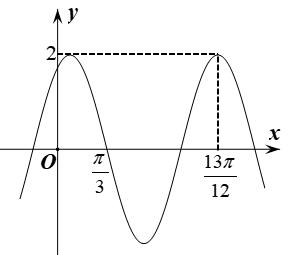
\includegraphics[width=.42\linewidth]{assets/asset-056-01.jpg}
\end{center}
\fillin[{$-\sqrt{3}$}]
\begin{solution}
\textbf{答案：}$-\sqrt{3}$

\textbf{分析：}首先确定函数的解析式，然后求解 $f\left(\frac{\pi}{2}\right)$ 的值即可.

\textbf{详解：}由题意可得：$\frac{3}{4}T = \frac{13\pi}{12} - \frac{\pi}{3} = \frac{3\pi}{4}$, 所以 $T = \pi$, $\omega = \frac{2\pi}{T} = 2$. 当 $x = \frac{13\pi}{12}$ 时，$\omega x + \varphi = 2 \times \frac{13\pi}{12} + \varphi = 2k\pi$, 所以 $\varphi = 2k\pi - \frac{13\pi}{6}$ ($k \in \mathbf{Z}$). 令 $k=1$ 可得：$\varphi = -\frac{\pi}{6}$. 据此有：$f(x) = 2\cos\left(2x - \frac{\pi}{6}\right)$, $f\left(\frac{\pi}{2}\right) = 2\cos\left(2\times\frac{\pi}{2} - \frac{\pi}{6}\right) = 2\cos\frac{5\pi}{6} = -\sqrt{3}$.
\end{solution}
\end{question}

\begin{question}[points=5]
\textbf{来源：}2021 年 全国乙卷-理科，第 7 题\par
把函数$y=f(x)$图像上所有点的横坐标缩短到原来的$\frac12$倍，纵坐标不变，再把所得曲线向右平移$\frac{\pi}{3}$个单位长度，得到函数$y=\sin\left(x-\frac{\pi}{4}\right)$的图像，则$f(x)=$（  ）
\begin{choices}
  \item $\sin\left(\frac{x}{2}-\frac{7\pi}{12}\right)$
  \item $\sin\left(\frac{x}{2}+\frac{\pi}{12}\right)$
  \item $\sin\left(2x-\frac{7\pi}{12}\right)$
  \item $\sin\left(2x+\frac{\pi}{12}\right)$
\end{choices}
\begin{solution}
\textbf{答案：}$\sin\left(\frac{x}{2}+\frac{\pi}{12}\right)$

\textbf{详解：}逆向：$y=\sin\left(x-\frac{\pi}{4}\right) \xrightarrow{\text{左移}\frac{\pi}{3}} y=\sin\left(x+\frac{\pi}{12}\right) \xrightarrow{\text{横坐标变为原来的2倍}} y=\sin\left(\frac{x}{2}+\frac{\pi}{12}\right)$。故选B。
\end{solution}
\end{question}

\begin{question}[points=5]
\textbf{来源：}2021 年 全国乙卷-文科，第 4 题\par
函数 $f(x) = \sin\frac{x}{3} + \cos\frac{x}{3}$ 的最小正周期和最大值分别是（ ）
\begin{choices}
  \item $3\pi$ 和 $\sqrt{2}$
  \item $3\pi$ 和 $2$
  \item $6\pi$ 和 $\sqrt{2}$
  \item $6\pi$ 和 $2$
\end{choices}
\begin{solution}
\textbf{答案：}C

\textbf{分析：}$f(x) = \sqrt{2}\sin\left(\frac{x}{3} + \frac{\pi}{4}\right)$ ，$f(x)_{\max} = \sqrt{2}$ ， $T = \frac{2\pi}{\frac{1}{3}} = 6\pi$ .
\end{solution}
\end{question}

\begin{question}[points=5]
\textbf{来源：}2021 年 全国乙卷-文科，第 6 题\par
$\cos^2\frac{\pi}{12} - \cos^2\frac{5\pi}{12} =$ （ ）
\begin{choices}
  \item $\frac{1}{2}$
  \item $\frac{\sqrt{3}}{3}$
  \item $\frac{\sqrt{2}}{2}$
  \item $\frac{\sqrt{3}}{2}$
\end{choices}
\begin{solution}
\textbf{答案：}D

\textbf{分析：}$\cos^2\frac{\pi}{12} - \cos^2\frac{5\pi}{12} = \cos^2\frac{\pi}{12} - \cos^2\left(\frac{\pi}{2} - \frac{\pi}{12}\right) = \cos^2\frac{\pi}{12} - \sin^2\frac{\pi}{12} = \cos\frac{\pi}{6} = \frac{\sqrt{3}}{2}$ .
\end{solution}
\end{question}

\begin{question}[points=5]
\textbf{来源：}2021 年 上海春季卷，第 12 题\par
已知 $\theta>0$，存在实数 $\varphi$，使得对任意 $n\in\mathbb{N}^*$，$\cos(n\theta+\varphi)<\frac{\sqrt{3}}{2}$，则 $\theta$ 的最小值是  .
\fillin[{$\frac{2\pi}{5}$}]
\begin{solution}
\textbf{答案：}$\frac{2\pi}{5}$

\textbf{分析：}在单位圆中分析可得 $\theta>\frac{\pi}{3}$，由 $\frac{2\pi}{\theta}\in\mathbb{N}^*$，即 $\theta=\frac{2\pi}{k}$，$k\in\mathbb{N}^*$，即可求得 $\theta$ 的最小值．

\textbf{详解：}在单位圆中分析，由题意可得 $n\theta+\varphi$ 的终边要落在图中阴影部分区域（其中 $\angle AOx=\angle BOx=\frac{\pi}{6}$），所以 $\theta>\angle AOB=\frac{\pi}{3}$，因为对任意 $n\in\mathbb{N}^*$ 都成立，所以 $\frac{2\pi}{\theta}\in\mathbb{N}^*$，即 $\theta=\frac{2\pi}{k}$，$k\in\mathbb{N}^*$，同时 $\theta>\frac{\pi}{3}$，所以 $\theta$ 的最小值为 $\frac{2\pi}{5}$．
\end{solution}
\end{question}

\begin{question}[points=5]
\textbf{来源：}2021 年 上海卷，第 15 题\par
已知$f(x)=3\sin x+2$，对于任意的$x_2\in[0,\frac{\pi}{2}]$，都存在$x_1\in[0,\frac{\pi}{2}]$，使得$f(x_1)+2f(x_2+\theta)=3$成立，则下列选项中，$\theta$可能的值是（\_\_\_\_\_\_）
\begin{choices}
  \item $\frac{3\pi}{5}$
  \item $\frac{4\pi}{5}$
  \item $\frac{6\pi}{5}$
  \item $\frac{7\pi}{5}$
\end{choices}
\begin{solution}
\textbf{答案：}D

\textbf{分析：}注意仔细审题，关注关键词“任意的”、“都存在”；

\textbf{详解：}由题设$f(x_1)+2f(x_2+\theta)=3$，变形得$f(x_1)=3-2f(x_2+\theta)$，又$f(x_1)\in[2,5]$，$y=3-2f(x_2+\theta)=-1-6\sin(x_2+\theta)$，当$\theta=\frac{7\pi}{5}$时，$x_2+\theta\in[\frac{7\pi}{5},\frac{19\pi}{10}]$，$y\in[1-6\sin\frac{19\pi}{10},5]$，而$1-6\sin\frac{19\pi}{10}\approx0.85<2$符合题意
\end{solution}
\end{question}

\begin{question}[points=5]
\textbf{来源：}2021 年 新高考I卷，第 4 题\par
下列区间中, 函数 $f(x) = 7\sin\left(x - \frac{\pi}{6}\right)$ 单调递增的区间是 ( )
\begin{choices}
  \item $\left(0, \frac{\pi}{2}\right)$
  \item $\left(\frac{\pi}{2}, \pi\right)$
  \item $\left(\pi, \frac{3\pi}{2}\right)$
  \item $\left(\frac{3\pi}{2}, 2\pi\right)$
\end{choices}
\begin{solution}
\textbf{答案：}$\left(0, \frac{\pi}{2}\right)$

\textbf{分析：}解不等式 $2k\pi - \frac{\pi}{2} < x - \frac{\pi}{6} < 2k\pi + \frac{\pi}{2} (k \in \mathbb{Z})$, 利用赋值法可得出结论.

\textbf{详解：}因为函数 $y = \sin x$ 的单调递增区间为 $\left(2k\pi - \frac{\pi}{2}, 2k\pi + \frac{\pi}{2}\right) (k \in \mathbb{Z})$, 对于函数 $f(x) = 7\sin\left(x - \frac{\pi}{6}\right)$, 由 $2k\pi - \frac{\pi}{2} < x - \frac{\pi}{6} < 2k\pi + \frac{\pi}{2}$, 解得 $2k\pi - \frac{\pi}{3} < x < 2k\pi + \frac{2\pi}{3}$. 取 $k=0$, 得一个单调递增区间为 $\left(-\frac{\pi}{3}, \frac{2\pi}{3}\right)$. 因为 $\left(0, \frac{\pi}{2}\right) \subset \left(-\frac{\pi}{3}, \frac{2\pi}{3}\right)$, 故选A.
\end{solution}
\end{question}

\begin{question}[points=5]
\textbf{来源：}2021 年 新高考I卷，第 6 题\par
若 $\tan\theta = -2$, 则 $\frac{\sin\theta(1 + \sin2\theta)}{\sin\theta + \cos\theta} =$ ( )
\begin{choices}
  \item $-\frac{6}{5}$
  \item $-\frac{2}{5}$
  \item $\frac{2}{5}$
  \item $\frac{6}{5}$
\end{choices}
\begin{solution}
\textbf{答案：}$\frac{2}{5}$

\textbf{分析：}将式子进行齐次化处理, 代入 $\tan\theta = -2$ 即可.

\textbf{详解：}$\frac{\sin\theta(1 + \sin2\theta)}{\sin\theta + \cos\theta} = \frac{\sin\theta(\sin^2\theta + \cos^2\theta + 2\sin\theta\cos\theta)}{\sin\theta + \cos\theta} = \sin\theta(\sin\theta + \cos\theta) = \frac{\sin\theta(\sin\theta + \cos\theta)}{\sin^2\theta + \cos^2\theta} = \frac{\tan^2\theta + \tan\theta}{1 + \tan^2\theta} = \frac{4 - 2}{1 + 4} = \frac{2}{5}$, 故选C.
\end{solution}
\end{question}

\begin{question}[points=4]
\textbf{来源：}2021 年 浙江卷，第 8 题\par
已知 $\alpha,\beta,\gamma$ 是互不相同的锐角, 则在 $\sin\alpha\cos\beta$, $\sin\beta\cos\gamma$, $\sin\gamma\cos\alpha$ 三个值中, 大于 $\frac{1}{2}$ 的个数的最大值是（   ）
\begin{choices}
  \item $0$
  \item $1$
  \item $2$
  \item $3$
\end{choices}
\begin{solution}
\textbf{答案：}C

\textbf{分析：}利用基本不等式或排序不等式得 $\sin\alpha\cos\beta+\sin\beta\cos\gamma+\sin\gamma\cos\alpha \leq \frac{3}{2}$, 从而可判断三个代数式不可能均大于 $\frac{1}{2}$, 再结合特例可得最大值.

\textbf{详解：}由基本不等式, $\sin\alpha\cos\beta \leq \frac{\sin^2\alpha+\cos^2\beta}{2}$, 同理可得和 $\leq \frac{3}{2}$, 故不可能三个都大于 $\frac{1}{2}$. 取 $\alpha=\frac{\pi}{6},\beta=\frac{\pi}{3},\gamma=\frac{\pi}{4}$, 则 $\sin\alpha\cos\beta = \frac{1}{4}<\frac{1}{2}$, $\sin\beta\cos\gamma = \frac{\sqrt{6}}{4}>\frac{1}{2}$, $\sin\gamma\cos\alpha = \frac{\sqrt{6}}{4}>\frac{1}{2}$, 故最大个数为2.
\end{solution}
\end{question}

\begin{question}[points=14]
\textbf{来源：}2021 年 浙江卷，第 18 题\par
设函数 $f(x)=\sin x+\cos x$ $(x\in\mathbb{R})$.

(1) 求函数 $y=\left[f\left(x+\frac{\pi}{2}\right)\right]^2$ 的最小正周期；

(2) 求函数 $y=f(x)f\left(x-\frac{\pi}{4}\right)$ 在 $[0,\frac{\pi}{2}]$ 上的最大值.
\begin{solution}
\textbf{答案：}(1) $\pi$; (2) $1+\frac{\sqrt{2}}{2}$

\textbf{分析：}(1) 利用三角恒等变换化简, 再求周期; (2) 化简表达式, 利用正弦函数的性质求最大值.

\textbf{详解：}(1) $f(x)=\sqrt{2}\sin\left(x+\frac{\pi}{4}\right)$, 则 $y=\left[\sqrt{2}\sin\left(x+\frac{3\pi}{4}\right)\right]^2=2\sin^2\left(x+\frac{3\pi}{4}\right)=1-\cos(2x+\frac{3\pi}{2})=1-\sin2x$, 故最小正周期 $T=\frac{2\pi}{2}=\pi$.
(2) $y=f(x)f(x-\frac{\pi}{4})=\sqrt{2}\sin(x+\frac{\pi}{4})\cdot\sqrt{2}\sin x = 2\sin x\cdot\frac{\sqrt{2}}{2}(\sin x+\cos x) = \sqrt{2}\sin^2 x + \sqrt{2}\sin x\cos x = \frac{\sqrt{2}}{2}(1-\cos2x) + \frac{\sqrt{2}}{2}\sin2x = \sin(2x-\frac{\pi}{4})+\frac{\sqrt{2}}{2}$. 当 $x\in[0,\frac{\pi}{2}]$ 时, $2x-\frac{\pi}{4}\in[-\frac{\pi}{4},\frac{3\pi}{4}]$, 故当 $2x-\frac{\pi}{4}=\frac{\pi}{2}$ 即 $x=\frac{3\pi}{8}$ 时, $y$ 取最大值 $1+\frac{\sqrt{2}}{2}$.
\end{solution}
\end{question}

\section*{2022 年}

\begin{question}[points=4]
\textbf{来源：}2022 年 北京卷，第 5 题\par
已知函数 $f(x) = \cos^2 x - \sin^2 x$，则
\begin{choices}
  \item $f(x)$ 在 $\left(-\dfrac{\pi}{2}, -\dfrac{\pi}{6}\right)$ 上单调递减
  \item $f(x)$ 在 $\left(-\dfrac{\pi}{4}, \dfrac{\pi}{12}\right)$ 上单调递增
  \item $f(x)$ 在 $\left(0, \dfrac{\pi}{3}\right)$ 上单调递减
  \item $f(x)$ 在 $\left(\dfrac{\pi}{4}, \dfrac{7\pi}{12}\right)$ 上单调递增
\end{choices}
\begin{solution}
\textbf{答案：}C

\textbf{分析：}化简得出 $f(x) = \cos 2x$，利用余弦型函数的单调性逐项判断。

\textbf{详解：}因为 $f(x) = \cos^2 x - \sin^2 x = \cos 2x$。
对于A，当 $-\dfrac{\pi}{2} < x < -\dfrac{\pi}{6}$ 时，$-\pi < 2x < -\dfrac{\pi}{3}$，则 $f(x)$ 在 $\left(-\dfrac{\pi}{2}, -\dfrac{\pi}{6}\right)$ 上单调递增，A错；
对于B，当 $-\dfrac{\pi}{4} < x < \dfrac{\pi}{12}$ 时，$-\dfrac{\pi}{2} < 2x < \dfrac{\pi}{6}$，则 $f(x)$ 在 $\left(-\dfrac{\pi}{4}, \dfrac{\pi}{12}\right)$ 上不单调，B错；
对于C，当 $0 < x < \dfrac{\pi}{3}$ 时，$0 < 2x < \dfrac{2\pi}{3}$，则 $f(x)$ 在 $\left(0, \dfrac{\pi}{3}\right)$ 上单调递减，C对；
对于D，当 $\dfrac{\pi}{4} < x < \dfrac{7\pi}{12}$ 时，$\dfrac{\pi}{2} < 2x < \dfrac{7\pi}{6}$，则 $f(x)$ 在 $\left(\dfrac{\pi}{4}, \dfrac{7\pi}{12}\right)$ 上不单调，D错。故选C。
\end{solution}
\end{question}

\begin{question}[points=5]
\textbf{来源：}2022 年 北京卷，第 13 题\par
若函数 $f(x) = A\sin x - \sqrt{3}\cos x$ 的一个零点为 $\dfrac{\pi}{3}$，则 $A =$ ；$f\left(\dfrac{\pi}{12}\right) =$ 。
\fillin[{$1$；$-\sqrt{2}$}]
\begin{solution}
\textbf{答案：}$1$；$-\sqrt{2}$

\textbf{分析：}先代入零点，求得 $A$ 的值，再将函数化简为 $f(x) = 2\sin\left(x - \dfrac{\pi}{3}\right)$，代入自变量 $x = \dfrac{\pi}{12}$ 计算。

\textbf{详解：}解：$\because f\left(\dfrac{\pi}{3}\right) = \dfrac{\sqrt{3}}{2}A - \dfrac{\sqrt{3}}{2} = 0$，$\therefore A = 1$。
$\therefore f(x) = \sin x - \sqrt{3}\cos x = 2\sin\left(x - \dfrac{\pi}{3}\right)$，
$f\left(\dfrac{\pi}{12}\right) = 2\sin\left(\dfrac{\pi}{12} - \dfrac{\pi}{3}\right) = 2\sin\left(-\dfrac{\pi}{4}\right) = -\sqrt{2}$。
\end{solution}
\end{question}

\begin{question}[points=5]
\textbf{来源：}2022 年 全国甲卷-理科，第 11 题\par
设函数 $f(x)=\sin\left(\omega x+\frac{\pi}{3}\right)$ 在区间 $(0,\pi)$ 恰有三个极值点、两个零点，则 $\omega$ 的取值范围是（ ）
\begin{choices}
  \item $\left[\frac{5}{3},\frac{13}{6}\right)$
  \item $\left[\frac{5}{3},\frac{19}{6}\right)$
  \item $\left(\frac{13}{6},\frac{8}{3}\right]$
  \item $\left(\frac{13}{6},\frac{19}{6}\right]$
\end{choices}
\begin{solution}
\textbf{答案：}C

\textbf{分析：}由x的取值范围得到$\omega x+\frac{\pi}{3}$的取值范围，再结合正弦函数的性质得到不等式组，解得即可.

\textbf{详解：}依题意可得$\omega>0$，因为$x\in(0,\pi)$，所以$\omega x+\frac{\pi}{3}\in\left(\frac{\pi}{3},\omega\pi+\frac{\pi}{3}\right)$，要使函数在区间$(0,\pi)$恰有三个极值点、两个零点，又$y=\sin x$, $x\in\left(\frac{\pi}{3},3\pi\right)$的图象如图所示，则$\frac{5\pi}{2}<\omega\pi+\frac{\pi}{3}\leq 3\pi$，解得$\frac{13}{6}<\omega\leq\frac{8}{3}$，即$\omega\in\left(\frac{13}{6},\frac{8}{3}\right]$. 故选C.
\end{solution}
\end{question}

\begin{question}[points=5]
\textbf{来源：}2022 年 全国甲卷-理科，第 12 题\par
已知 $a=\frac{31}{32}$, $b=\cos\frac{1}{4}$, $c=4\sin\frac{1}{4}$，则（ ）
\begin{choices}
  \item $c>b>a$
  \item $b>a>c$
  \item $a>b>c$
  \item $a>c>b$
\end{choices}
\begin{solution}
\textbf{答案：}A

\textbf{分析：}由$\frac{c}{b}=4\tan\frac{1}{4}$结合三角函数的性质可得$c>b$；构造函数$f(x)=\cos x+\frac{1}{2}x^2-1, x\in(0,+\infty)$，利用导数可得$b>a$，即可得解.

\textbf{详解：}因为当$x\in(0,\frac{\pi}{2})$时，$x<\tan x$，故$\frac{c}{b}=4\tan\frac{1}{4}>1$，所以$c>b$；设$f(x)=\cos x+\frac{1}{2}x^2-1$, $x\in(0,+\infty)$，$f'(x)=-\sin x+x>0$，所以$f(x)$在$(0,+\infty)$单调递增，故$f(\frac{1}{4})>f(0)=0$，所以$\cos\frac{1}{4}-\frac{31}{32}>0$，所以$b>a$，因此$c>b>a$. 故选A.
\end{solution}
\end{question}

\begin{question}[points=5]
\textbf{来源：}2022 年 全国甲卷-文科，第 5 题\par
将函数 $f(x)=\sin\left(\omega x+\frac{\pi}{3}\right) (\omega>0)$ 的图像向左平移 $\frac{\pi}{2}$ 个单位长度后得到曲线 $C$，若 $C$ 关于 $y$ 轴对称，则 $\omega$ 的最小值是
\begin{choices}
  \item $\frac{1}{6}$
  \item $\frac{1}{4}$
  \item $\frac{1}{3}$
  \item $\frac{1}{2}$
\end{choices}
\begin{solution}
\textbf{答案：}C
\end{solution}
\end{question}

\begin{question}[points=5]
\textbf{来源：}2022 年 全国乙卷-理科，第 15 题\par
记函数$f(x) = \cos(\omega x + \varphi)$ $(\omega > 0, 0 < \varphi < \pi)$的最小正周期为$T$，若$f(T) = \frac{\sqrt{3}}{2}$，且$x = \frac{\pi}{9}$为$f(x)$的零点，则$\omega$的最小值为．
\fillin[{$3$}]
\begin{solution}
\textbf{答案：}$3$

\textbf{分析：}首先表示出$T$，根据$f(T)=\frac{\sqrt{3}}{2}$求出$\varphi$，再根据$x=\frac{\pi}{9}$为函数的零点，即可求出$\omega$的取值，从而得解；

\textbf{详解：}解：因为$f(x)=\cos(\omega x+\varphi)$，$(\omega>0,0<\varphi<\pi)$所以最小正周期$T=\frac{2\pi}{\omega}$，因为$f(T)=\cos\left(\omega\cdot\frac{2\pi}{\omega}+\varphi\right)=\cos(2\pi+\varphi)=\cos\varphi=\frac{\sqrt{3}}{2}$，又$0<\varphi<\pi$，所以$\varphi=\frac{\pi}{6}$，即$f(x)=\cos\left(\omega x+\frac{\pi}{6}\right)$，又$x=\frac{\pi}{9}$为$f(x)$的零点，所以$\frac{\pi}{9}\omega+\frac{\pi}{6}=\frac{\pi}{2}+k\pi, k\in\mathbb{Z}$，解得$\omega=3+9k, k\in\mathbb{Z}$，因为$\omega>0$，所以当$k=0$时$\omega_{\min}=3$；
\end{solution}
\end{question}

\begin{question}[points=4]
\textbf{来源：}2022 年 上海卷，第 2 题\par
函数$f(x) = \cos^2 x - \sin^2 x + 1$的周期为 ．
\fillin[{$\pi$}]
\begin{solution}
\textbf{答案：}$\pi$

\textbf{分析：}由三角函数的恒等变换化简函数可得$f(x)=\cos 2x+1$，从而根据周期公式即可求值．

\textbf{详解：}解：$f(x)=\cos^2 x - \sin^2 x + 1 = \cos 2x + 1$，$T=\frac{2\pi}{2}=\pi$．故答案为：$\pi$．
\end{solution}
\end{question}

\begin{question}[points=5]
\textbf{来源：}2022 年 天津卷，第 9 题\par
已知 $f(x)=\frac{1}{2}\sin 2x$，关于该函数有下列四个说法：① $f(x)$ 的最小正周期为 $2\pi$；② $f(x)$ 在 $[-\frac{\pi}{4},\frac{\pi}{4}]$ 上单调递增；③当 $x\in[-\frac{\pi}{6},\frac{\pi}{3}]$ 时，$f(x)$ 的取值范围为 $[-\frac{\sqrt{3}}{4},\frac{\sqrt{3}}{4}]$；④ $f(x)$ 的图象可由 $g(x)=\frac{1}{2}\sin(2x+\frac{\pi}{4})$ 的图象向左平移 $\frac{\pi}{8}$ 个单位长度得到．以上四个说法中，正确的个数为（   ）
\begin{choices}
  \item 1
  \item 2
  \item 3
  \item 4
\end{choices}
\begin{solution}
\textbf{答案：}1

\textbf{分析：}因为 $f(x)=\frac{1}{2}\sin 2x$，所以最小正周期为 $T=\frac{2\pi}{2}=\pi$，①不正确；令 $t=2x\in[-\frac{\pi}{2},\frac{\pi}{2}]$，而 $y=\frac{1}{2}\sin t$ 在 $[-\frac{\pi}{2},\frac{\pi}{2}]$ 上递增，所以 $f(x)$ 在 $[-\frac{\pi}{4},\frac{\pi}{4}]$ 上单调递增，②正确；因为 $t=2x\in[-\frac{\pi}{3},\frac{2\pi}{3}]$，$\sin t\in[-\frac{\sqrt{3}}{2},1]$，所以 $f(x)\in[-\frac{\sqrt{3}}{4},\frac{1}{2}]$，③不正确；由于 $g(x)=\frac{1}{2}\sin(2x+\frac{\pi}{4})=\frac{1}{2}\sin[2(x+\frac{\pi}{8})]$，所以 $f(x)$ 的图象可由 $g(x)$ 的图象向右平移 $\frac{\pi}{8}$ 个单位长度得到，④不正确．故选 A.
\end{solution}
\end{question}

\begin{question}[points=5]
\textbf{来源：}2022 年 新高考II卷，第 6 题\par
若 $\sin(\alpha+\beta)+\cos(\alpha+\beta)=2\sqrt{2}\cos\left(\alpha+\dfrac{\pi}{4}\right)\sin\beta$，则（ ）
\begin{choices}
  \item $\tan(\alpha-\beta)=1$
  \item $\tan(\alpha+\beta)=1$
  \item $\tan(\alpha-\beta)=-1$
  \item $\tan(\alpha+\beta)=-1$
\end{choices}
\begin{solution}
\textbf{答案：}$\tan(\alpha-\beta)=-1$

\textbf{分析：}由两角和差的正余弦公式化简，结合同角三角函数的商数关系即可得解.

\textbf{详解：}由已知得：$\sin\alpha\cos\beta+\cos\alpha\sin\beta+\cos\alpha\cos\beta-\sin\alpha\sin\beta=2(\cos\alpha-\sin\alpha)\sin\beta$，即$\sin\alpha\cos\beta-\cos\alpha\sin\beta+\cos\alpha\cos\beta+\sin\alpha\sin\beta=0$，即$\sin(\alpha-\beta)+\cos(\alpha-\beta)=0$，所以$\tan(\alpha-\beta)=-1$，故选C.
\end{solution}
\end{question}

\begin{question}[points=5]
\textbf{来源：}2022 年 新高考II卷，第 9 题\par
已知函数$f(x)=\sin(2x+\varphi)(0<\varphi<\pi)$的图像关于点$\left(\dfrac{2\pi}{3},0\right)$中心对称，则（ ）
\begin{choices}
  \item $f(x)$在区间$\left(0,\dfrac{5\pi}{12}\right)$单调递减
  \item $f(x)$在区间$\left(-\dfrac{\pi}{12},\dfrac{11\pi}{12}\right)$有两个极值点
  \item 直线$x=\dfrac{7\pi}{6}$是曲线$y=f(x)$的对称轴
  \item 直线$y=\dfrac{\sqrt{3}}{2}-x$是曲线$y=f(x)$的切线
\end{choices}
\begin{solution}
\textbf{答案：}AD

\textbf{分析：}根据三角函数的性质逐个判断各选项，即可解出.

\textbf{详解：}由题意得$f\left(\dfrac{2\pi}{3}\right)=\sin\left(\dfrac{4\pi}{3}+\varphi\right)=0$，所以$\dfrac{4\pi}{3}+\varphi=k\pi,k\in\mathbf{Z}$，即$\varphi=-\dfrac{4\pi}{3}+k\pi,k\in\mathbf{Z}$，又$0<\varphi<\pi$，所以$k=2$时，$\varphi=\dfrac{2\pi}{3}$，故$f(x)=\sin\left(2x+\dfrac{2\pi}{3}\right)$．对A，当$x\in\left(0,\dfrac{5\pi}{12}\right)$时，$2x+\dfrac{2\pi}{3}\in\left(\dfrac{2\pi}{3},\dfrac{3\pi}{2}\right)$，由正弦函数$y=\sin u$图象知$y=f(x)$在$\left(0,\dfrac{5\pi}{12}\right)$上是单调递减；对B，当$x\in\left(-\dfrac{\pi}{12},\dfrac{11\pi}{12}\right)$时，$2x+\dfrac{2\pi}{3}\in\left(\dfrac{\pi}{2},\dfrac{5\pi}{2}\right)$，由正弦函数$y=\sin u$图象知$y=f(x)$只有1个极值点，由$2x+\dfrac{2\pi}{3}=\dfrac{3\pi}{2}$，解得$x=\dfrac{5\pi}{12}$，即$x=\dfrac{5\pi}{12}$为函数的唯一极值点；对C，当$x=\dfrac{7\pi}{6}$时，$2x+\dfrac{2\pi}{3}=3\pi$，$f\left(\dfrac{7\pi}{6}\right)=0$，直线$x=\dfrac{7\pi}{6}$不是对称轴；对D，由$y'=2\cos\left(2x+\dfrac{2\pi}{3}\right)=-1$得$\cos\left(2x+\dfrac{2\pi}{3}\right)=-\dfrac{1}{2}$，解得$2x+\dfrac{2\pi}{3}=\dfrac{2\pi}{3}+2k\pi$或$2x+\dfrac{2\pi}{3}=\dfrac{4\pi}{3}+2k\pi,k\in\mathbf{Z}$，从而得$x=k\pi$或$x=\dfrac{\pi}{3}+k\pi,k\in\mathbf{Z}$，所以函数$y=f(x)$在点$\left(0,\dfrac{\sqrt{3}}{2}\right)$处的切线斜率为$k=y'|_{x=0}=2\cos\dfrac{2\pi}{3}=-1$，切线方程为$y-\dfrac{\sqrt{3}}{2}=-(x-0)$即$y=\dfrac{\sqrt{3}}{2}-x$．故选AD.
\end{solution}
\end{question}

\begin{question}[points=5]
\textbf{来源：}2022 年 新高考I卷，第 6 题\par
记函数 $f(x) = \sin\left(\omega x + \frac{\pi}{4}\right) + b\ (\omega > 0)$ 的最小正周期为 $T$. 若 $\frac{2\pi}{3} < T < \pi$, 且 $y = f(x)$ 的图象关于点 $\left(\frac{3\pi}{2}, 2\right)$ 中心对称, 则 $f\left(\frac{\pi}{2}\right) =$
\begin{choices}
  \item $1$
  \item $\frac{3}{2}$
  \item $\frac{5}{2}$
  \item $3$
\end{choices}
\begin{solution}
\textbf{答案：}A

\textbf{分析：}由三角函数的图象与性质可求得参数, 进而可得函数解析式, 代入即可得解.

\textbf{详解：}由函数的最小正周期 $T$ 满足 $\frac{2\pi}{3} < T < \pi$, 得 $\frac{2\pi}{3} < \frac{2\pi}{\omega} < \pi$, 解得 $2 < \omega < 3$. 又因为函数图象关于点 $\left(\frac{3\pi}{2}, 2\right)$ 对称, 所以 $\omega \cdot \frac{3\pi}{2} + \frac{\pi}{4} = k\pi$, $k \in \mathbb{Z}$, 且 $b = 2$. 所以 $\omega = -\frac{1}{6} + \frac{2}{3}k$, $k \in \mathbb{Z}$, 所以 $\omega = \frac{5}{2}$, $f(x) = \sin\left(\frac{5}{2}x + \frac{\pi}{4}\right) + 2$. 所以 $f\left(\frac{\pi}{2}\right) = \sin\left(\frac{5}{4}\pi + \frac{\pi}{4}\right) + 2 = 1$.
\end{solution}
\end{question}

\begin{question}[points=4]
\textbf{来源：}2022 年 浙江卷，第 6 题\par
为了得到函数 $y = 2\sin 3x$ 的图象，只要把函数 $y = 2\sin\left(3x + \frac{\pi}{5}\right)$ 图象上所有的点（ ）
\begin{choices}
  \item 向左平移 $\dfrac{\pi}{5}$ 个单位长度
  \item 向右平移 $\dfrac{\pi}{5}$ 个单位长度
  \item 向左平移 $\dfrac{\pi}{15}$ 个单位长度
  \item 向右平移 $\dfrac{\pi}{15}$ 个单位长度
\end{choices}
\begin{solution}
\textbf{答案：}D

\textbf{分析：}根据三角函数图象的变换法则即可求出．

\textbf{详解：}$y = 2\sin 3x = 2\sin\left[3\left(x - \frac{\pi}{15}\right) + \frac{\pi}{5}\right]$，所以向右平移 $\frac{\pi}{15}$ 个单位长度，故选D.
\end{solution}
\end{question}

\begin{question}[points=6]
\textbf{来源：}2022 年 浙江卷，第 13 题\par
若 $3\sin\alpha - \sin\beta = \sqrt{10}$，$\alpha+\beta = \dfrac{\pi}{2}$，则 $\sin\alpha =$ ，$\cos 2\beta =$ ．
\fillin[{$\dfrac{3\sqrt{10}}{10}$；$\dfrac{4}{5}$}]
\begin{solution}
\textbf{答案：}$\dfrac{3\sqrt{10}}{10}$；$\dfrac{4}{5}$

\textbf{分析：}先通过诱导公式变形，得到 $\alpha$ 的同角等式关系，再利用辅助角公式化简成正弦型函数方程，可求出 $\alpha$，接下来再求 $\beta$．

\textbf{详解：}由 $\alpha+\beta=\frac{\pi}{2}$ 得 $\sin\beta = \cos\alpha$，代入得 $3\sin\alpha - \cos\alpha = \sqrt{10}$，即 $\sqrt{10}\sin(\alpha-\theta)=\sqrt{10}$，其中 $\sin\theta=\frac{1}{\sqrt{10}}$，$\cos\theta=\frac{3}{\sqrt{10}}$，所以 $\alpha-\theta = \frac{\pi}{2}+2k\pi$，$\sin\alpha = \sin(\theta+\frac{\pi}{2}) = \cos\theta = \frac{3\sqrt{10}}{10}$，$\cos2\beta = 2\cos^2\beta-1 = 2\sin^2\alpha-1 = \frac{4}{5}$.
\end{solution}
\end{question}

\section*{2023 年}

\begin{question}[points=5]
\textbf{来源：}2023 年 北京卷，第 13 题\par
已知命题 $p$ : 若 $\alpha, \beta$ 为第一象限角，且 $\alpha > \beta$ ，则 $\tan \alpha > \tan \beta$ ．能说明 $p$ 为假命题的一组 $\alpha, \beta$ 的值为 $\alpha =$ ， $\beta =$ ．
\fillin[{$\dfrac{9\pi}{4}$ ; $\dfrac{\pi}{3}$}]
\begin{solution}
\textbf{答案：}$\dfrac{9\pi}{4}$ ; $\dfrac{\pi}{3}$

\textbf{分析：}根据正切函数单调性以及任意角的定义分析求解.

\textbf{详解：}因为 $f(x)=\tan x$ 在 $(0,\frac{\pi}{2})$ 上单调递增，若 $0<\alpha_0<\beta_0<\frac{\pi}{2}$，则 $\tan\alpha_0<\tan\beta_0$，取 $\alpha=2k_1\pi+\alpha_0, \beta=2k_2\pi+\beta_0, k_1,k_2\in\mathbb{Z}$，则 $\tan\alpha=\tan\alpha_0, \tan\beta=\tan\beta_0$，即 $\tan\alpha<\tan\beta$，令 $k_1>k_2$，则 $\alpha-\beta=2(k_1-k_2)\pi+(\alpha_0-\beta_0)>0$，即 $\alpha>\beta$。不妨取 $k_1=1,k_2=0,\alpha_0=\frac{\pi}{4},\beta_0=\frac{\pi}{3}$，即 $\alpha=\frac{9\pi}{4},\beta=\frac{\pi}{3}$ 满足题意。
\end{solution}
\end{question}

\begin{question}[points=13]
\textbf{来源：}2023 年 北京卷，第 17 题\par
设函数 $f(x) = \sin\omega x\cos\varphi + \cos\omega x\sin\varphi$ $\left(\omega>0, |\varphi|<\dfrac{\pi}{2}\right)$．

（1）若 $f(0) = -\dfrac{\sqrt{3}}{2}$ ，求 $\varphi$ 的值．

（2）已知 $f(x)$ 在区间 $\left[-\dfrac{\pi}{3}, \dfrac{2\pi}{3}\right]$ 上单调递增， $f\left(\dfrac{2\pi}{3}\right)=1$ ，再从条件①、条件②、条件③这三个条件中选择一个作为已知，使函数 $f(x)$ 存在，求 $\omega, \varphi$ 的值．

条件①：$f\left(\dfrac{\pi}{3}\right)=\sqrt{2}$；

条件②：$f\left(-\dfrac{\pi}{3}\right)=-1$；

条件③：$f(x)$ 在区间 $\left[-\dfrac{\pi}{2}, -\dfrac{\pi}{3}\right]$ 上单调递减．

注：如果选择的条件不符合要求，第（2）问得0分；如果选择多个符合要求的条件分别解答，按第一个解答计分．
\begin{solution}
\textbf{答案：}（1）$\varphi=-\dfrac{\pi}{3}$ （2）条件①不能使函数$f(x)$存在；条件②或条件③可解得$\omega=1$，$\varphi=-\dfrac{\pi}{6}$

\textbf{分析：}（1）把$x=0$代入$f(x)$的解析式求出$\sin\varphi$，再由$|\varphi|<\frac{\pi}{2}$即可求出$\varphi$的值；（2）若选条件①不合题意；若选条件②，先把$f(x)$的解析式化简，根据$f(x)$在$[-\frac{\pi}{3},\frac{2\pi}{3}]$上的单调性及函数的最值可求出$T$，从而求出$\omega$的值；把$\omega$的值代入$f(x)$的解析式，由$f(-\frac{\pi}{3})=-1$和$|\varphi|<\frac{\pi}{2}$即可求出$\varphi$的值；若选条件③：由$f(x)$的单调性可知$f(x)$在$x=-\frac{\pi}{3}$处取得最小值$-1$，则与条件②所给的条件一样，解法与条件②相同.

\textbf{详解：}（1）因为 $f(x)=\sin\omega x\cos\varphi+\cos\omega x\sin\varphi$, $\omega>0$, $|\varphi|<\frac{\pi}{2}$，所以 $f(0)=\sin0\cos\varphi+\cos0\sin\varphi=\sin\varphi=-\frac{\sqrt{3}}{2}$，因为 $|\varphi|<\frac{\pi}{2}$，所以 $\varphi=-\frac{\pi}{3}$。
（2）$f(x)=\sin(\omega x+\varphi)$，$\omega>0$, $|\varphi|<\frac{\pi}{2}$，所以 $f(x)$ 的最大值为1，最小值为-1。若选条件①：因为 $f(x)$ 的最大值为1，最小值为-1，所以 $f(\frac{\pi}{3})=\sqrt{2}$ 无解，故条件①不能使函数 $f(x)$ 存在；若选条件②：因为 $f(x)$ 在 $[-\frac{\pi}{3},\frac{2\pi}{3}]$ 上单调递增，且 $f(\frac{2\pi}{3})=1$，$f(-\frac{\pi}{3})=-1$，所以 $\frac{T}{2}=\frac{2\pi}{3}-(-\frac{\pi}{3})=\pi$，所以 $T=2\pi$，$\omega=\frac{2\pi}{T}=1$，所以 $f(x)=\sin(x+\varphi)$，又因为 $f(-\frac{\pi}{3})=-1$，所以 $\sin(-\frac{\pi}{3}+\varphi)=-1$，所以 $-\frac{\pi}{3}+\varphi=-\frac{\pi}{2}+2k\pi$，$k\in\mathbb{Z}$，所以 $\varphi=-\frac{\pi}{6}+2k\pi$，因为 $|\varphi|<\frac{\pi}{2}$，所以 $\varphi=-\frac{\pi}{6}$。所以 $\omega=1$，$\varphi=-\frac{\pi}{6}$；若选条件③：因为 $f(x)$ 在 $[-\frac{\pi}{3},\frac{2\pi}{3}]$ 上单调递增，在 $[-\frac{\pi}{2},-\frac{\pi}{3}]$ 上单调递减，所以 $f(x)$ 在 $x=-\frac{\pi}{3}$ 处取得最小值 $-1$，即 $f(-\frac{\pi}{3})=-1$。以下与条件②相同。
\end{solution}
\end{question}

\begin{question}[points=5]
\textbf{来源：}2023 年 全国甲卷-理科，第 10 题\par
函数 $y = f(x)$ 的图象由函数 $y = \cos\left(2x + \frac{\pi}{6}\right)$ 的图象向左平移 $\frac{\pi}{6}$ 个单位长度得到，则 $y = f(x)$ 的图象与直线 $y = \frac{1}{2}x - \frac{1}{2}$ 的交点个数为（                  ）
\begin{choices}
  \item $1$
  \item $2$
  \item $3$
  \item $4$
\end{choices}
\begin{solution}
\textbf{答案：}C

\textbf{分析：}先利用三角函数平移的性质求得 $f(x) = -\sin 2x$，再作出 $f(x)$ 与 $y = \frac{1}{2}x - \frac{1}{2}$ 的部分大致图像，考虑特殊点处 $f(x)$ 与 $y = \frac{1}{2}x - \frac{1}{2}$ 的大小关系，从而精确图像，由此得解．

\textbf{详解：}因为 $y = \cos\left(2x + \frac{\pi}{6}\right)$ 向左平移 $\frac{\pi}{6}$ 个单位所得函数为 $y = \cos\left[2\left(x + \frac{\pi}{6}\right) + \frac{\pi}{6}\right] = \cos\left(2x + \frac{\pi}{2}\right) = -\sin 2x$，所以 $f(x) = -\sin 2x$，而 $y = \frac{1}{2}x - \frac{1}{2}$ 显然过 $(0, -\frac{1}{2})$ 与 $(1,0)$ 两点，作出 $f(x)$ 与 $y = \frac{1}{2}x - \frac{1}{2}$ 的部分大致图像如下，考虑 $2x = -\frac{3\pi}{2}, 2x = \frac{3\pi}{2}, 2x = \frac{7\pi}{2}$，即 $x = -\frac{3\pi}{4}, x = \frac{3\pi}{4}, x = \frac{7\pi}{4}$ 处 $f(x)$ 与 $y = \frac{1}{2}x - \frac{1}{2}$ 的大小关系，当 $x = -\frac{3\pi}{4}$ 时，$f(-\frac{3\pi}{4}) = -\sin\left(-\frac{3\pi}{2}\right) = -1$，$y = \frac{1}{2}\times\left(-\frac{3\pi}{4}\right) - \frac{1}{2} = -\frac{3\pi+4}{8} < -1$；当 $x = \frac{3\pi}{4}$ 时，$f(\frac{3\pi}{4}) = -\sin\frac{3\pi}{2} = 1$，$y = \frac{1}{2}\times\frac{3\pi}{4} - \frac{1}{2} = \frac{3\pi-4}{8} < 1$；当 $x = \frac{7\pi}{4}$ 时，$f(\frac{7\pi}{4}) = -\sin\frac{7\pi}{2} = 1$，$y = \frac{1}{2}\times\frac{7\pi}{4} - \frac{1}{2} = \frac{7\pi-4}{8} > 1$；所以由图可知，$f(x)$ 与 $y = \frac{1}{2}x - \frac{1}{2}$ 的交点个数为 3．
\end{solution}
\end{question}

\begin{question}[points=5]
\textbf{来源：}2023 年 全国甲卷-文科，第 12 题\par
函数 $y=f(x)$ 的图象由 $y=\cos\left(2x+\frac{\pi}{6}\right)$ 的图象向左平移 $\frac{\pi}{6}$ 个单位长度得到，则 $y=f(x)$ 的图象与直线 $y=\frac{1}{2}x-\frac{1}{2}$ 的交点个数为（    ）
\begin{choices}
  \item $1$
  \item $2$
  \item $3$
  \item $4$
\end{choices}
\begin{solution}
\textbf{答案：}C

\textbf{分析：}先利用三角函数平移的性质求得 $f(x)=-\sin2x$，再作出 $f(x)$ 与 $y=\frac{1}{2}x-\frac{1}{2}$ 的部分大致图像，考虑特殊点处 $f(x)$ 与 $y=\frac{1}{2}x-\frac{1}{2}$ 的大小关系，从而精确图像，由此得解.

\textbf{详解：}因为 $y=\cos\left(2x+\frac{\pi}{6}\right)$ 向左平移 $\frac{\pi}{6}$ 个单位所得函数为 $y=\cos\left[2(x+\frac{\pi}{6})+\frac{\pi}{6}\right]=\cos\left(2x+\frac{\pi}{2}\right)=-\sin2x$，所以 $f(x)=-\sin2x$，而 $y=\frac{1}{2}x-\frac{1}{2}$ 显然过 $(0,-\frac{1}{2})$ 与 $(1,0)$ 两点，作出 $f(x)$ 与 $y=\frac{1}{2}x-\frac{1}{2}$ 的部分大致图像，考虑 $2x=-\frac{3\pi}{2},2x=\frac{3\pi}{2},2x=\frac{7\pi}{2}$，即 $x=-\frac{3\pi}{4},x=\frac{3\pi}{4},x=\frac{7\pi}{4}$ 处 $f(x)$ 与 $y=\frac{1}{2}x-\frac{1}{2}$ 的大小关系，当 $x=-\frac{3\pi}{4}$ 时，$f(-\frac{3\pi}{4})=-\sin(-\frac{3\pi}{2})=-1$，$y=\frac{1}{2}\times(-\frac{3\pi}{4})-\frac{1}{2}=-\frac{3\pi+4}{8}<-1$；当 $x=\frac{3\pi}{4}$ 时，$f(\frac{3\pi}{4})=-\sin\frac{3\pi}{2}=1$，$y=\frac{1}{2}\times\frac{3\pi}{4}-\frac{1}{2}=\frac{3\pi-4}{8}<1$；当 $x=\frac{7\pi}{4}$ 时，$f(\frac{7\pi}{4})=-\sin\frac{7\pi}{2}=1$，$y=\frac{1}{2}\times\frac{7\pi}{4}-\frac{1}{2}=\frac{7\pi-4}{8}>1$；所以由图可知，$f(x)$ 与 $y=\frac{1}{2}x-\frac{1}{2}$ 的交点个数为3，故选C.
\end{solution}
\end{question}

\begin{question}[points=5]
\textbf{来源：}2023 年 全国乙卷-理科，第 6 题\par
已知函数 $f(x)=\sin(\omega x+\varphi)$ 在区间 $(\frac{\pi}{6},\frac{2\pi}{3})$ 单调递增，直线 $x=\frac{\pi}{6}$ 和 $x=\frac{2\pi}{3}$ 为函数 $y=f(x)$ 的图像的两条对称轴，则 $f(-\frac{5\pi}{12})=$（ ）
\begin{choices}
  \item $-\frac{\sqrt{3}}{2}$
  \item $-\frac{1}{2}$
  \item $\frac{1}{2}$
  \item $\frac{\sqrt{3}}{2}$
\end{choices}
\begin{solution}
\textbf{答案：}$\frac{\sqrt{3}}{2}$

\textbf{分析：}根据题意分别求出其周期，再根据其最小值求出初相，代入 $x=-\frac{5\pi}{12}$ 即可得到答案.

\textbf{详解：}因为 $f(x)=\sin(\omega x+\varphi)$ 在区间 $(\frac{\pi}{6},\frac{2\pi}{3})$ 单调递增，所以 $\frac{T}{2}=\frac{2\pi}{3}-\frac{\pi}{6}=\frac{\pi}{2}$，且 $\omega>0$，则 $T=\pi$，$\omega=\frac{2\pi}{T}=2$，当 $x=\frac{\pi}{6}$ 时，$f(x)$ 取得最小值，则 $2\cdot\frac{\pi}{6}+\varphi=2k\pi-\frac{\pi}{2}$，$k\in\mathbb{Z}$，则 $\varphi=2k\pi-\frac{5\pi}{6}$，$k\in\mathbb{Z}$，不妨取 $k=0$，则 $f(x)=\sin(2x-\frac{5\pi}{6})$，则 $f(-\frac{5\pi}{12})=\sin(-\frac{5\pi}{3})=\frac{\sqrt{3}}{2}$.
\end{solution}
\end{question}

\begin{question}[points=5]
\textbf{来源：}2023 年 全国乙卷-文科，第 10 题\par
已知函数$f(x)=\sin(\omega x+\varphi)$在区间$(\frac{\pi}{6},\frac{2\pi}{3})$单调递增，直线$x=\frac{\pi}{6}$和$x=\frac{2\pi}{3}$为函数$y=f(x)$的图像的两条对称轴，则$f(-\frac{5\pi}{12})=$（   ）
\begin{choices}
  \item -$\frac{\sqrt{3}}{2}$
  \item -$\frac{1}{2}$
  \item $\frac{1}{2}$
  \item $\frac{\sqrt{3}}{2}$
\end{choices}
\begin{solution}
\textbf{答案：}$\frac{\sqrt{3}}{2}$

\textbf{分析：}根据题意分别求出其周期，再根据其最小值求出初相，代入$x=-\frac{5\pi}{12}$即可得到答案.

\textbf{详解：}因为$f(x)=\sin(\omega x+\varphi)$在区间$(\frac{\pi}{6},\frac{2\pi}{3})$单调递增，所以$\frac{T}{2}=\frac{2\pi}{3}-\frac{\pi}{6}=\frac{\pi}{2}$，且$\omega>0$，则$T=\pi$，$\omega=\frac{2\pi}{T}=2$，当$x=\frac{\pi}{6}$时，$f(x)$取得最小值，则$2\cdot\frac{\pi}{6}+\varphi=2k\pi-\frac{\pi}{2}$，$k\in \mathbb{Z}$，则$\varphi=2k\pi-\frac{5\pi}{6}$，$k\in \mathbb{Z}$，不妨取$k=0$，则$f(x)=\sin(2x-\frac{5\pi}{6})$，则$f(-\frac{5\pi}{12})=\sin(-\frac{5\pi}{3})=\frac{\sqrt{3}}{2}$. 故选D.
\end{solution}
\end{question}

\begin{question}[points=5]
\textbf{来源：}2023 年 全国乙卷-文科，第 14 题\par
若$\theta\in(0,\frac{\pi}{2})$，$\tan\theta=\frac{1}{2}$，则$\sin\theta-\cos\theta=$.
\fillin[{$-\frac{\sqrt{5}}{5}$}]
\begin{solution}
\textbf{答案：}$-\frac{\sqrt{5}}{5}$

\textbf{分析：}根据同角三角关系求$\sin\theta$，进而可得结果.

\textbf{详解：}因为$\theta\in(0,\frac{\pi}{2})$，则$\sin\theta>0, \cos\theta>0$，又因为$\tan\theta=\frac{\sin\theta}{\cos\theta}=\frac{1}{2}$，则$\cos\theta=2\sin\theta$，且$\cos^2\theta+\sin^2\theta=4\sin^2\theta+\sin^2\theta=5\sin^2\theta=1$，解得$\sin\theta=\frac{\sqrt{5}}{5}$或$\sin\theta=-\frac{\sqrt{5}}{5}$（舍去），所以$\sin\theta-\cos\theta=\sin\theta-2\sin\theta=-\sin\theta=-\frac{\sqrt{5}}{5}$. 故答案为$-\frac{\sqrt{5}}{5}$.
\end{solution}
\end{question}

\begin{question}[points=4]
\textbf{来源：}2023 年 上海卷，第 4 题\par
已知 $\tan \alpha = 2$，求 $\frac{\sin \alpha - \cos \alpha}{\sin \alpha + \cos \alpha}=$
\fillin[{$\frac{1}{3}$}]
\begin{solution}
\textbf{答案：}$\frac{1}{3}$
\end{solution}
\end{question}

\begin{question}[points=5]
\textbf{来源：}2023 年 上海卷，第 11 题；次专题：一元二次函数、方程和不等式\par
公园修建斜坡,假设斜坡起点在水平面上,斜坡与水平面的夹角为 $\theta$,斜坡终点距离水平面的垂直高度为4米,游客每走一米消耗的体能为 $1+\sin \theta$,要使游客从斜坡底走到斜坡顶端所消耗的总体能最少,则 $\tan \theta=$
\fillin[{$\frac{1}{2}$}]
\begin{solution}
\textbf{答案：}$\frac{1}{2}$
\end{solution}
\end{question}

\begin{question}[points=5]
\textbf{来源：}2023 年 天津卷，第 5 题\par
已知函数 $f(x)$ 的一条对称轴为直线 $x = 2$, 一个周期为 $4$, 则 $f(x)$ 的解析式可能为 ( )
\begin{choices}
  \item $\sin\left(\dfrac{\pi}{2}x\right)$
  \item $\cos\left(\dfrac{\pi}{2}x\right)$
  \item $\sin\left(\dfrac{\pi}{4}x\right)$
  \item $\cos\left(\dfrac{\pi}{4}x\right)$
\end{choices}
\begin{solution}
\textbf{答案：}B

\textbf{分析：}由题意分别考查函数的最小正周期和函数在 $x=2$ 处的函数值.

\textbf{详解：}A 选项 $T = \dfrac{2\pi}{\pi/2} = 4$, B 选项 $T = \dfrac{2\pi}{\pi/2} = 4$, C 选项 $T = \dfrac{2\pi}{\pi/4} = 8$, D 选项 $T = \dfrac{2\pi}{\pi/4} = 8$, 排除 CD. 对于 A, 当 $x=2$ 时 $\sin\left(\dfrac{\pi}{2}\cdot 2\right)=0$, 故 $(2,0)$ 是一个对称中心, 排除 A. 对于 B, 当 $x=2$ 时 $\cos\left(\dfrac{\pi}{2}\cdot 2\right) = -1$, 故 $x=2$ 是一条对称轴. 故选 B.
\end{solution}
\end{question}

\begin{question}[points=5]
\textbf{来源：}2023 年 新高考II卷，第 7 题\par
已知$\alpha$为锐角，$\cos\alpha=\dfrac{1+\sqrt{5}}{4}$，则$\sin\dfrac{\alpha}{2}=$（ \quad ）
\begin{choices}
  \item A. $\dfrac{3-\sqrt{5}}{8}$
  \item B. $\dfrac{-1+\sqrt{5}}{8}$
  \item C. $\dfrac{3-\sqrt{5}}{4}$
  \item D. $\dfrac{-1+\sqrt{5}}{4}$
\end{choices}
\begin{solution}
\textbf{答案：}D

\textbf{分析：}根据二倍角公式（或者半角公式）即可求出.

\textbf{详解：}因为$\cos\alpha=1-2\sin^{2}\dfrac{\alpha}{2}=\dfrac{1+\sqrt{5}}{4}$，而$\alpha$为锐角，解得$\sin\dfrac{\alpha}{2}=\dfrac{3-\sqrt{5}}{8}=\dfrac{(\sqrt{5}-1)^{2}}{16}=\dfrac{\sqrt{5}-1}{4}$.
\end{solution}
\end{question}

\begin{question}[points=5]
\textbf{来源：}2023 年 新高考II卷，第 16 题\par
已知函数$f(x)=\sin(\omega x+\varphi)$，如图$A$，$B$是直线$y=\dfrac{1}{2}$与曲线$y=f(x)$的两个交点，若$|AB|=\dfrac{\pi}{6}$，则$f(\pi)=$ ．

\begin{center}
  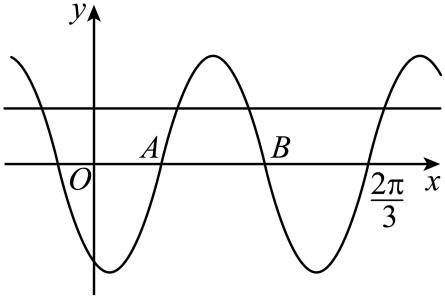
\includegraphics[width=.42\linewidth]{assets/asset-090-01.jpg}
\end{center}
\fillin[{$-\dfrac{\sqrt{3}}{2}$}]
\begin{solution}
\textbf{答案：}$-\dfrac{\sqrt{3}}{2}$

\textbf{分析：}设$A\left(x_{1},\dfrac{1}{2}\right),B\left(x_{2},\dfrac{1}{2}\right)$，依题可得$x_{2}-x_{1}=\dfrac{\pi}{6}$，结合$\sin x=\dfrac{1}{2}$的解可得$\omega(x_{2}-x_{1})=\dfrac{2\pi}{3}$，从而得到$\omega$的值，再根据$f\left(\dfrac{2\pi}{3}\right)=0$以及$f(0)<0$，即可得$f(x)=\sin\left(4x-\dfrac{2\pi}{3}\right)$，进而求得$f(\pi)$.

\textbf{详解：}设$A\left(x_{1},\dfrac{1}{2}\right),B\left(x_{2},\dfrac{1}{2}\right)$，由$|AB|=\dfrac{\pi}{6}$可得$x_{2}-x_{1}=\dfrac{\pi}{6}$，由$\sin x=\dfrac{1}{2}$可知，$x=\dfrac{\pi}{6}+2k\pi$或$x=\dfrac{5\pi}{6}+2k\pi$，$k\in\mathbb{Z}$，由图可知，$\omega x_{2}+\varphi-(\omega x_{1}+\varphi)=\dfrac{5\pi}{6}-\dfrac{\pi}{6}=\dfrac{2\pi}{3}$，即$\omega(x_{2}-x_{1})=\dfrac{2\pi}{3}$，$\therefore\omega=4$. 因为$f\left(\dfrac{2\pi}{3}\right)=\sin\left(\dfrac{8\pi}{3}+\varphi\right)=0$，所以$\dfrac{8\pi}{3}+\varphi=k\pi$，即$\varphi=-\dfrac{8\pi}{3}+k\pi$，$k\in\mathbb{Z}$. 所以$f(x)=\sin\left(4x-\dfrac{8\pi}{3}+k\pi\right)=\sin\left(4x-\dfrac{2\pi}{3}+k\pi\right)$，所以$f(x)=\sin\left(4x-\dfrac{2\pi}{3}\right)$或$f(x)=-\sin\left(4x-\dfrac{2\pi}{3}\right)$，又因为$f(0)<0$，所以$f(x)=\sin\left(4x-\dfrac{2\pi}{3}\right)$，$\therefore f(\pi)=\sin\left(4\pi-\dfrac{2\pi}{3}\right)=-\dfrac{\sqrt{3}}{2}$.
\end{solution}
\end{question}

\begin{question}[points=5]
\textbf{来源：}2023 年 新高考I卷，第 8 题\par
已知 $\sin(\alpha-\beta)=\frac{1}{3},\cos\alpha\sin\beta=\frac{1}{6}$，则 $\cos(2\alpha+2\beta)=$（ ）
\begin{choices}
  \item $\frac{7}{9}$
  \item $\frac{1}{9}$
  \item $-\frac{1}{9}$
  \item $-\frac{7}{9}$
\end{choices}
\begin{solution}
\textbf{答案：}$\frac{1}{9}$

\textbf{分析：}根据给定条件，利用和角、差角的正弦公式求出 $\sin(\alpha+\beta)$，再利用二倍角的余弦公式计算作答。

\textbf{详解：}因为 $\sin(\alpha-\beta)=\sin\alpha\cos\beta-\cos\alpha\sin\beta=\frac{1}{3}$，而 $\cos\alpha\sin\beta=\frac{1}{6}$，因此 $\sin\alpha\cos\beta=\frac{1}{2}$，则 $\sin(\alpha+\beta)=\sin\alpha\cos\beta+\cos\alpha\sin\beta=\frac{2}{3}$，所以 $\cos(2\alpha+2\beta)=\cos2(\alpha+\beta)=1-2\sin^2(\alpha+\beta)=1-2\times(\frac{2}{3})^2=\frac{1}{9}$。
\end{solution}
\end{question}

\begin{question}[points=5]
\textbf{来源：}2023 年 新高考I卷，第 15 题\par
已知函数 $f(x)=\cos\omega x-1(\omega>0)$ 在区间 $[0,2\pi]$ 有且仅有 3 个零点，则 $\omega$ 的取值范围是．
\fillin[{$[2,3)$}]
\begin{solution}
\textbf{答案：}$[2,3)$

\textbf{分析：}令 $f(x)=0$，得 $\cos\omega x=1$ 有 3 个根，从而结合余弦函数的图像性质即可得解。

\textbf{详解：}因为 $0\leq x\leq 2\pi$，所以 $0\leq \omega x\leq 2\omega\pi$，令 $f(x)=\cos\omega x-1=0$，则 $\cos\omega x=1$ 有 3 个根，令 $t=\omega x$，则 $\cos t=1$ 有 3 个根，其中 $t\in[0,2\omega\pi]$，结合余弦函数 $y=\cos t$ 的图像性质可得 $4\pi\leq 2\omega\pi < 6\pi$，故 $2\leq \omega < 3$。
\end{solution}
\end{question}

\section*{2024 年}

\begin{question}[points=4]
\textbf{来源：}2024 年 北京卷，第 6 题\par
已知 $f(x)=\sin\omega x(\omega>0)$，$f(x_1)=-1$，$f(x_2)=1$，$|x_1-x_2|_{\min}=\dfrac{\pi}{2}$，则 $\omega=$ （ ）
\begin{choices}
  \item $1$
  \item $2$
  \item $3$
  \item $4$
\end{choices}
\begin{solution}
\textbf{答案：}B

\textbf{分析：}根据三角函数最值分析周期性，结合三角函数最小正周期公式运算求解。

\textbf{详解：}由题意可知：$x_1$ 为 $f(x)$ 的最小值点，$x_2$ 为 $f(x)$ 的最大值点，则 $|x_1-x_2|_{\min}=\dfrac{T}{2}=\dfrac{\pi}{2}$，即 $T=\pi$，且 $\omega>0$，所以 $\omega=\dfrac{2\pi}{T}=2$。故选：B。
\end{solution}
\end{question}

\begin{question}[points=5]
\textbf{来源：}2024 年 北京卷，第 12 题\par
已知 $\alpha \in \left[\dfrac{\pi}{6},\dfrac{\pi}{3}\right]$，且 $\alpha$ 与 $\beta$ 的终边关于原点对称，则 $\cos \beta$ 的最大值为。
\fillin[{$-\dfrac{1}{2}$}]
\begin{solution}
\textbf{答案：}$-\dfrac{1}{2}$

\textbf{分析：}首先得出 $\beta = \alpha + \pi + 2k\pi, k \in \mathbb{Z}$，结合三角函数单调性即可求解最值。

\textbf{详解：}由题意 $\beta = \alpha + \pi + 2k\pi, k \in \mathbb{Z}$，从而 $\cos \beta = \cos(\alpha+\pi+2k\pi) = -\cos \alpha$。因为 $\alpha \in [\dfrac{\pi}{6},\dfrac{\pi}{3}]$，所以 $\cos \alpha \in [\dfrac{1}{2},\dfrac{\sqrt{3}}{2}]$，$\cos \beta \in [-\dfrac{\sqrt{3}}{2},-\dfrac{1}{2}]$。当且仅当 $\alpha = \dfrac{\pi}{3}$，即 $\beta = \dfrac{4\pi}{3} + 2k\pi, k \in \mathbb{Z}$ 时，$\cos \beta$ 取得最大值，且最大值为 $-\dfrac{1}{2}$。
\end{solution}
\end{question}

\begin{question}[points=5]
\textbf{来源：}2024 年 全国甲卷-理科，第 8 题\par
已知 $\dfrac{\cos\alpha}{\cos\alpha-\sin\alpha}=3$，则 $\tan\left(\alpha+\dfrac{\pi}{4}\right)=$ （   ）
\begin{choices}
  \item $2\sqrt{3}+1$
  \item $2\sqrt{3}-1$
  \item $\dfrac{3}{2}$
  \item $1-\sqrt{3}$
\end{choices}
\begin{solution}
\textbf{答案：}B

\textbf{分析：}先将 $\dfrac{\cos\alpha}{\cos\alpha-\sin\alpha}$ 弦化切求得 $\tan\alpha$，再根据两角和的正切公式即可求解。

\textbf{详解：}因为 $\dfrac{\cos\alpha}{\cos\alpha-\sin\alpha}=3$，所以 $\dfrac{1}{1-\tan\alpha}=3$，$\Rightarrow\tan\alpha=1-\frac{1}{3}$，所以 $\tan\left(\alpha+\frac{\pi}{4}\right)=\frac{\tan\alpha+1}{1-\tan\alpha}=2\sqrt{3}-1$。
\end{solution}
\end{question}

\begin{question}[points=5]
\textbf{来源：}2024 年 全国甲卷-文科，第 9 题\par
已知 $\frac{\cos\alpha}{\cos\alpha - \sin\alpha} = 3$，则 $\tan\left(\alpha + \frac{\pi}{4}\right) =$（ ）
\begin{choices}
  \item $2\sqrt{3} + 1$
  \item $2\sqrt{3} - 1$
  \item $\frac{\sqrt{3}}{2}$
  \item $1 - \sqrt{3}$
\end{choices}
\begin{solution}
\textbf{答案：}B

\textbf{分析：}先将 $\frac{\cos\alpha}{\cos\alpha - \sin\alpha}$ 弦化切求得 $\tan\alpha$，再根据两角和的正切公式即可求解.

\textbf{详解：}因为 $\frac{\cos\alpha}{\cos\alpha - \sin\alpha} = \sqrt{3}$（原卷可能为 $\sqrt{3}$，但文本层显示为3，解析版中也处理为 $\sqrt{3}$），所以 $\frac{1}{1 - \tan\alpha} = \sqrt{3}$，$\Rightarrow \tan\alpha = 1 - \frac{1}{\sqrt{3}} = \frac{\sqrt{3} - 1}{\sqrt{3}}$，所以 $\tan\left(\alpha + \frac{\pi}{4}\right) = \frac{\tan\alpha + 1}{1 - \tan\alpha} = \frac{\frac{\sqrt{3} - 1}{\sqrt{3}} + 1}{1 - \frac{\sqrt{3} - 1}{\sqrt{3}}} = \frac{\frac{2\sqrt{3} - 1}{\sqrt{3}}}{\frac{1}{\sqrt{3}}} = 2\sqrt{3} - 1$.
\end{solution}
\end{question}

\begin{question}[points=5]
\textbf{来源：}2024 年 全国甲卷-文科，第 12 题\par
函数 $f(x) = \sin x - \sqrt{3} \cos x$ 在 $[0, \pi]$ 上的最大值是．
\fillin[{$2$}]
\begin{solution}
\textbf{答案：}$2$

\textbf{分析：}结合辅助角公式化简成正弦型函数，再求给定区间最值即可.

\textbf{详解：}$f(x) = \sin x - \sqrt{3} \cos x = 2\sin\left(x - \frac{\pi}{3}\right)$，当 $x \in [0, \pi]$ 时，$x - \frac{\pi}{3} \in [-\frac{\pi}{3}, \frac{2\pi}{3}]$，当 $x - \frac{\pi}{3} = \frac{\pi}{2}$ 即 $x = \frac{5\pi}{6}$ 时，$f(x)_{\max} = 2$.
\end{solution}
\end{question}

\begin{question}[points=4]
\textbf{来源：}2024 年 上海卷，第 14 题\par
下列函数$f(x)$的最小正周期是$2\pi$的是（\quad\quad）
\begin{choices}
  \item $A\ \sin x+\cos x$
  \item $B\ \sin x\cos x$
  \item $C\ \sin^2x+\cos^2x$
  \item $D\ \sin^2x-\cos^2x$
\end{choices}
\begin{solution}
\textbf{答案：}$A$

\textbf{分析：}根据辅助角公式、二倍角公式以及同角三角函数关系并结合三角函数的性质一一判断即可.

\textbf{详解：}对A，$\sin x+\cos x=\sqrt{2}\sin\left(x+\frac{\pi}{4}\right)$，周期$T=2\pi$，故A正确；对B，$\sin x\cos x=\frac{1}{2}\sin2x$，周期$T=\frac{2\pi}{2}=\pi$，故B错误；对于选项C，$\sin^2x+\cos^2x=1$，是常值函数，不存在最小正周期，故C错误；对于选项D，$\sin^2x-\cos^2x=-\cos2x$，周期$T=\frac{2\pi}{2}=\pi$，故D错误，故选：A.
\end{solution}
\end{question}

\begin{question}[points=5]
\textbf{来源：}2024 年 天津卷，第 7 题\par
已知函数 $f(x)=\sin^3\left(\omega x + \frac{\pi}{3}\right) (\omega>0)$ 的最小正周期为 $\pi$. 则函数在 $\left[-\frac{\pi}{12},\frac{\pi}{6}\right]$ 的最小值是 ( )
\begin{choices}
  \item $-\frac{\sqrt{3}}{2}$
  \item $-\frac{3}{2}$
  \item $0$
  \item $\frac{\sqrt{3}}{2}$
\end{choices}
\begin{solution}
\textbf{答案：}$-\frac{\sqrt{3}}{2}$

\textbf{分析：}先由诱导公式化简, 结合周期公式求出 $\omega$, 得 $f(x)=-\sin 2x$, 再整体求出 $x\in\left[-\frac{\pi}{12},\frac{\pi}{6}\right]$ 时 $2x$ 的范围, 结合正弦三角函数图象特征即可求解.

\textbf{详解：}$f(x)=\sin^3\left(\omega x+\frac{\pi}{3}\right)=\sin(3\omega x+\pi)=-\sin 3\omega x$, 由 $T=\frac{2\pi}{3\omega}=\pi$ 得 $\omega=\frac{2}{3}$, 即 $f(x)=-\sin 2x$. 当 $x\in\left[-\frac{\pi}{12},\frac{\pi}{6}\right]$ 时, $2x\in\left[-\frac{\pi}{6},\frac{\pi}{3}\right]$, 画出 $f(x)=-\sin 2x$ 图象, 由图可知 $f(x)=-\sin 2x$ 在 $\left[-\frac{\pi}{12},\frac{\pi}{6}\right]$ 上递减, 所以当 $x=\frac{\pi}{6}$ 时, $f(x)_{\min}=-\sin\frac{\pi}{3}=-\frac{\sqrt{3}}{2}$. 故选A.
\end{solution}
\end{question}

\begin{question}[points=6]
\textbf{来源：}2024 年 新高考II卷，第 9 题\par
对于函数$f(x)=\sin 2x$和$g(x)=\sin(2x-\dfrac{\pi}{4})$，下列正确的有（ ）
\begin{choices}
  \item $f(x)$与$g(x)$有相同零点
  \item $f(x)$与$g(x)$有相同最大值
  \item $f(x)$与$g(x)$有相同的最小正周期
  \item $f(x)$与$g(x)$的图像有相同的对称轴
\end{choices}
\begin{solution}
\textbf{答案：}$BC$

\textbf{分析：}根据正弦函数的零点、最值、周期公式、对称轴方程逐一分析每个选项即可.

\textbf{详解：}A选项，令$f(x)=\sin 2x=0$，解得$x=\dfrac{k\pi}{2},k\in\mathbb{Z}$，即为$f(x)$零点；令$g(x)=\sin(2x-\dfrac{\pi}{4})=0$，解得$x=\dfrac{k\pi}{2}+\dfrac{\pi}{8},k\in\mathbb{Z}$，即为$g(x)$零点，显然$f(x),g(x)$零点不同，A选项错误。B选项，显然$f(x)_{\max}=g(x)_{\max}=1$，B选项正确。C选项，根据周期公式，$f(x),g(x)$的周期均为$\dfrac{2\pi}{2}=\pi$，C选项正确。D选项，根据正弦函数的性质$f(x)$的对称轴满足$2x=k\pi+\dfrac{\pi}{2}\Leftrightarrow x=\dfrac{k\pi}{2}+\dfrac{\pi}{4},k\in\mathbb{Z}$，$g(x)$的对称轴满足$2x-\dfrac{\pi}{4}=k\pi+\dfrac{\pi}{2}\Leftrightarrow x=\dfrac{k\pi}{2}+\dfrac{3\pi}{8},k\in\mathbb{Z}$，显然$f(x),g(x)$图像的对称轴不同，D选项错误.
\end{solution}
\end{question}

\begin{question}[points=5]
\textbf{来源：}2024 年 新高考II卷，第 13 题\par
已知$\alpha$为第一象限角，$\beta$为第三象限角，$\tan\alpha+\tan\beta=4$，$\tan\alpha\tan\beta=\sqrt{2}+1$，则$\sin(\alpha+\beta)=$.
\fillin[{$-\dfrac{2\sqrt{2}}{3}$}]
\begin{solution}
\textbf{答案：}$-\dfrac{2\sqrt{2}}{3}$

\textbf{分析：}法一：根据两角和与差的正切公式得$\tan(\alpha+\beta)=-2\sqrt{2}$，再缩小$\alpha+\beta$的范围，最后结合同角的平方和关系即可得到答案；法二：利用弦化切的方法即可得到答案.

\textbf{详解：}法一：由题意得$\tan(\alpha+\beta)=\dfrac{\tan\alpha+\tan\beta}{1-\tan\alpha\tan\beta}=\dfrac{4}{1-(\sqrt{2}+1)}=-2\sqrt{2}$。因为$\alpha\in\left(2k\pi,2k\pi+\dfrac{\pi}{2}\right)$，$\beta\in\left(2m\pi+\pi,2m\pi+\dfrac{3\pi}{2}\right)$，$k,m\in\mathbb{Z}$，则$\alpha+\beta\in( (2m+2k)\pi+\pi, (2m+2k)\pi+2\pi )$，$k,m\in\mathbb{Z}$。又因为$\tan(\alpha+\beta)=-2\sqrt{2}<0$，则$\alpha+\beta\in\left( (2m+2k)\pi+\dfrac{3\pi}{2}, (2m+2k)\pi+2\pi\right)$，$k,m\in\mathbb{Z}$，则$\sin(\alpha+\beta)<0$。由$\dfrac{\sin(\alpha+\beta)}{\cos(\alpha+\beta)}=-2\sqrt{2}$，联立$\sin^2(\alpha+\beta)+\cos^2(\alpha+\beta)=1$，解得$\sin(\alpha+\beta)=-\dfrac{2\sqrt{2}}{3}$。法二：因为$\alpha$为第一象限角，$\beta$为第三象限角，则$\cos\alpha>0$，$\cos\beta<0$。$\cos\alpha=\dfrac{\cos\alpha}{\sin^2\alpha+\cos^2\alpha}=\dfrac{1}{\sqrt{1+\tan^2\alpha}}$，$\cos\beta=\dfrac{\cos\beta}{\sin^2\beta+\cos^2\beta}=\dfrac{-1}{\sqrt{1+\tan^2\beta}}$，则$\sin(\alpha+\beta)=\sin\alpha\cos\beta+\cos\alpha\sin\beta=\cos\alpha\cos\beta(\tan\alpha+\tan\beta)=4\cos\alpha\cos\beta=\dfrac{-4}{\sqrt{1+\tan^2\alpha}\sqrt{1+\tan^2\beta}}=\dfrac{-4}{\sqrt{(\tan\alpha+\tan\beta)^2+(\tan\alpha\tan\beta-1)^2}}=\dfrac{-4}{\sqrt{4^2+(\sqrt{2})^2}}=-\dfrac{2\sqrt{2}}{3}$.
\end{solution}
\end{question}

\begin{question}[points=5]
\textbf{来源：}2024 年 新高考I卷，第 4 题\par
已知 $\cos(\alpha+\beta)=m, \tan\alpha\tan\beta=2$，则 $\cos(\alpha-\beta)=$（ ）
\begin{choices}
  \item $-3m$
  \item $-\dfrac{m}{3}$
  \item $\dfrac{m}{3}$
  \item $3m$
\end{choices}
\begin{solution}
\textbf{答案：}A

\textbf{分析：}根据两角和的余弦可求 $\cos\alpha\cos\beta,\sin\alpha\sin\beta$ 的关系，结合 $\tan\alpha\tan\beta$ 的值可求前者，故可求 $\cos(\alpha-\beta)$ 的值.

\textbf{详解：}因为 $\cos(\alpha+\beta)=m$，所以 $\cos\alpha\cos\beta-\sin\alpha\sin\beta=m$，而 $\tan\alpha\tan\beta=2$，所以 $\sin\alpha\sin\beta=2\cos\alpha\cos\beta$，故 $\cos\alpha\cos\beta-2\cos\alpha\cos\beta=m$，即 $\cos\alpha\cos\beta=-m$，从而 $\sin\alpha\sin\beta=-2m$，故 $\cos(\alpha-\beta)=-3m$.
\end{solution}
\end{question}

\begin{question}[points=5]
\textbf{来源：}2024 年 新高考I卷，第 7 题\par
当 $x\in[0,2\pi]$ 时，曲线 $y=\sin x$ 与 $y=2\sin\left(3x-\dfrac{\pi}{6}\right)$ 的交点个数为（ ）

\begin{center}
  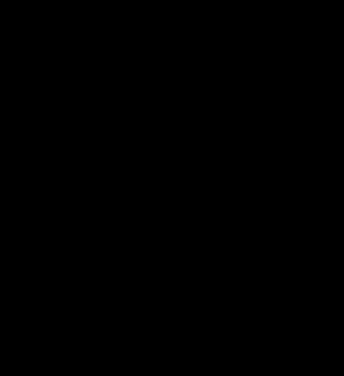
\includegraphics[width=.42\linewidth]{assets/asset-103-01.jpg}
\end{center}
\begin{choices}
  \item $3$
  \item $4$
  \item $6$
  \item $8$
\end{choices}
\begin{solution}
\textbf{答案：}C

\textbf{分析：}画出两函数在 $[0,2\pi]$ 上的图象，根据图象即可求解.

\textbf{详解：}因为函数 $y=\sin x$ 的最小正周期为 $T=2\pi$，函数 $y=2\sin\left(3x-\dfrac{\pi}{6}\right)$ 的最小正周期为 $T=\dfrac{2\pi}{3}$，所以在 $x\in[0,2\pi]$ 上函数 $y=2\sin\left(3x-\dfrac{\pi}{6}\right)$ 有三个周期的图象，在坐标系中结合五点法画出两函数图象，如图所示：由图可知，两函数图象有 6 个交点.
\end{solution}
\end{question}

\section*{2025 年}

\begin{question}[points=5]
\textbf{来源：}2025 年 全国II卷，第 8 题\par
已知 $0<\alpha<\pi$，$\cos\frac{\alpha}{2}=\frac{\sqrt{5}}{5}$，则 $\sin\left(\alpha-\frac{\pi}{4}\right)=$（ ）
\begin{choices}
  \item $\frac{\sqrt{2}}{10}$
  \item $\frac{\sqrt{2}}{5}$
  \item $\frac{3\sqrt{2}}{10}$
  \item $\frac{7\sqrt{2}}{10}$
\end{choices}
\begin{solution}
\textbf{答案：}$D$

\textbf{分析：}利用二倍角余弦公式得 $\cos\alpha=-\frac{3}{5}$，则 $\sin\alpha=\frac{4}{5}$，最后再根据两角差的正弦公式即可得到答案.

\textbf{详解：}$\cos\alpha=2\cos^2\frac{\alpha}{2}-1=2\times\left(\frac{\sqrt{5}}{5}\right)^2-1=-\frac{3}{5}$，因为 $0<\alpha<\pi$，则 $\frac{\pi}{2}<\alpha<\pi$，则 $\sin\alpha=\sqrt{1-\cos^2\alpha}=\sqrt{1-\left(-\frac{3}{5}\right)^2}=\frac{4}{5}$，则 $\sin\left(\alpha-\frac{\pi}{4}\right)=\sin\alpha\cos\frac{\pi}{4}-\cos\alpha\sin\frac{\pi}{4}=\frac{4}{5}\times\frac{\sqrt{2}}{2}-\left(-\frac{3}{5}\right)\times\frac{\sqrt{2}}{2}=\frac{7\sqrt{2}}{10}$.
\end{solution}
\end{question}

\begin{question}[points=13]
\textbf{来源：}2025 年 全国II卷，第 15 题\par
已知函数 $f(x)=\cos(2x+\varphi)$ $(0\le\varphi<\pi)$，$f(0)=\frac{1}{2}$.

（1）求 $\varphi$;

（2）设函数 $g(x)=f(x)+f\left(x-\frac{\pi}{6}\right)$，求 $g(x)$ 的值域和单调区间.
\begin{solution}
\textbf{答案：}（1）$\varphi=\frac{\pi}{3}$
（2）值域为 $[-\sqrt{3},\sqrt{3}]$；单调递减区间为 $[-\frac{\pi}{12}+k\pi,\frac{5\pi}{12}+k\pi]\ (k\in\mathbb{Z})$；单调递增区间为 $[\frac{5\pi}{12}+k\pi,\frac{11\pi}{12}+k\pi]\ (k\in\mathbb{Z})$.

\textbf{分析：}（1）直接由题意得 $\cos\varphi=\frac{1}{2},(0\le\varphi<\pi)$，结合余弦函数的单调性即可得解；（2）由三角恒等变换得 $g(x)=\sqrt{3}\cos\left(2x+\frac{\pi}{6}\right)$，由此可得值域，进一步由整体代入法可得函数的单调区间.

\textbf{详解：}（1）由题意 $f(0)=\cos\varphi=\frac{1}{2}$，且 $0\le\varphi<\pi$，所以 $\varphi=\frac{\pi}{3}$.
（2）由（1）可知 $f(x)=\cos\left(2x+\frac{\pi}{3}\right)$，所以 $g(x)=f(x)+f\left(x-\frac{\pi}{6}\right)=\cos\left(2x+\frac{\pi}{3}\right)+\cos2x=\frac{1}{2}\cos2x-\frac{\sqrt{3}}{2}\sin2x+\cos2x=\frac{3}{2}\cos2x-\frac{\sqrt{3}}{2}\sin2x=\sqrt{3}\cos\left(2x+\frac{\pi}{6}\right)$，所以函数 $g(x)$ 的值域为 $[-\sqrt{3},\sqrt{3}]$. 令 $2k\pi\le2x+\frac{\pi}{6}\le\pi+2k\pi,k\in\mathbb{Z}$，解得 $-\frac{\pi}{12}+k\pi\le x\le\frac{5\pi}{12}+k\pi,k\in\mathbb{Z}$；令 $\pi+2k\pi\le2x+\frac{\pi}{6}\le2\pi+2k\pi,k\in\mathbb{Z}$，解得 $\frac{5\pi}{12}+k\pi\le x\le\frac{11\pi}{12}+k\pi,k\in\mathbb{Z}$. 所以函数 $g(x)$ 的单调递减区间为 $[-\frac{\pi}{12}+k\pi,\frac{5\pi}{12}+k\pi]\ (k\in\mathbb{Z})$，单调递增区间为 $[\frac{5\pi}{12}+k\pi,\frac{11\pi}{12}+k\pi]\ (k\in\mathbb{Z})$.
\end{solution}
\end{question}

\begin{question}[points=5]
\textbf{来源：}2025 年 全国I卷，第 4 题\par
若点 $(a,0)(a>0)$ 是函数 $y = 2\tan\left(x - \frac{\pi}{3}\right)$ 的图象的一个对称中心，则 $a$ 的最小值为（ ）
\begin{choices}
  \item $\frac{\pi}{4}$
  \item $\frac{\pi}{2}$
  \item $\frac{\pi}{3}$
  \item $\frac{4\pi}{3}$
\end{choices}
\begin{solution}
\textbf{答案：}C

\textbf{分析：}根据正切函数的对称中心的结论求解.

\textbf{详解：}根据正切函数的性质，$y = 2\tan\left(x - \frac{\pi}{3}\right)$ 的对称中心横坐标满足 $x - \frac{\pi}{3} = \frac{k\pi}{2}, k \in \mathbb{Z}$，即对称中心是 $\left(\frac{\pi}{3} + \frac{k\pi}{2}, 0\right), k \in \mathbb{Z}$，即 $a = \frac{\pi}{3} + \frac{k\pi}{2}, k \in \mathbb{Z}$，又 $a>0$，则 $k=0$ 时 $a$ 最小，最小值是 $\frac{\pi}{3}$，即 $a = \frac{\pi}{3}$. 故选：C.
\end{solution}
\end{question}

\begin{question}[points=6]
\textbf{来源：}2025 年 全国I卷，第 11 题；次专题：平面向量与解三角形\par
已知 $\triangle ABC$ 的面积为 $\frac{1}{4}$，若 $\cos^2 A + \cos^2 B + 2\sin C = 2$，$\cos A \cos B \sin C = \frac{1}{4}$，则（ ）
\begin{choices}
  \item $\sin C = \sin^2 A + \sin^2 B$
  \item $AB = \sqrt{2}$
  \item $\sin A + \sin B = \frac{\sqrt{6}}{2}$
  \item $AC^2 + BC^2 = 3$
\end{choices}
\begin{solution}
\textbf{答案：}ABC

\textbf{分析：}对 $\cos^2 A + \cos^2 B + 2\sin C = 2$ 由二倍角公式先可推知 $\sin C = \sin^2 A + \sin^2 B$，然后分情况比较 $A+B$ 和 $\frac{\pi}{2}$ 的大小，结合正弦函数的单调性可推出 $C = \frac{\pi}{2}$，然后利用 $\cos A \cos B \sin C = \frac{1}{4}$ 算出 $A,B$ 取值，最后利用三角形面积求出三边长，即可判断每个选项.

\textbf{详解：}由 $\cos^2 A + \cos^2 B + 2\sin C = 2$ 得 $1-2\sin^2 A + 1-2\sin^2 B + 2\sin C = 2$，整理得 $\sin C = \sin^2 A + \sin^2 B$，A 正确；由正弦定理得 $a^2+b^2=c^2$，即 $C = \frac{\pi}{2}$，则 $\cos A \cos B = \frac{1}{4}$，又 $A+B=\frac{\pi}{2}$，所以 $\sin A \cos A = \frac{1}{4}$，即 $\sin 2A = \frac{1}{2}$，解得 $A = \frac{\pi}{12}, B = \frac{5\pi}{12}$，则 $\sin A + \sin B = \frac{\sqrt{6}-\sqrt{2}}{4} + \frac{\sqrt{6}+\sqrt{2}}{4} = \frac{\sqrt{6}}{2}$，C 正确；设 $BC = t$，则 $AC = (2+\sqrt{3})t$，$AB = (\sqrt{6}+\sqrt{2})t$，由面积公式 $\frac{1}{2} \cdot (2+\sqrt{3})t^2 = \frac{1}{4}$，解得 $t = \frac{\sqrt{3}-1}{2}$，则 $AB = (\sqrt{6}+\sqrt{2}) \cdot \frac{\sqrt{3}-1}{2} = \sqrt{2}$，B 正确；$AC^2+BC^2 = ((2+\sqrt{3})^2+1)t^2 = (8+4\sqrt{3}) \cdot \frac{(\sqrt{3}-1)^2}{4} = (8+4\sqrt{3}) \cdot \frac{4-2\sqrt{3}}{4} = (2+\sqrt{3})(4-2\sqrt{3}) = 2$，D 错误. 故选：ABC.
\end{solution}
\end{question}

\begin{question}[points=17]
\textbf{来源：}2025 年 全国I卷，第 19 题；次专题：导数\par
设函数 $f(x) = 5\cos x - \cos 5x$.



（1）求 $f(x)$ 在 $\left[0, \frac{\pi}{4}\right]$ 的最大值；



（2）给定 $\theta \in (0,\pi)$，设 $a$ 为实数，证明：存在 $y \in [a-\theta, a+\theta]$，使得 $\cos y \le \cos \theta$；



（3）若存在 $\varphi$ 使得对任意 $x$，都有 $|5\cos x - \cos(5x+\varphi)| \le b$，求 $b$ 的最小值.
\begin{solution}
\textbf{答案：}（1）$3\sqrt{3}$；（2）证明见解析；（3）$3\sqrt{3}$

\textbf{分析：}（1）利用导数结合三角变换得导数零点，讨论导数的符号后得单调性，从而可求最大值；或者利用均值不等式可求最大值.（2）利用反证法可证三角不等式有解；（3）先考虑 $t=0,\pi$ 时 $b$ 的范围，对于 $t \in (0,\pi)$ 时，可利用（2）中的结论结合特值法求得 $b \ge 3\sqrt{3}$，从而可得 $b$ 的最小值；或者先根据函数解析特征得 $b \ge 0$，再结合特值法可得 $b \ge 3\sqrt{3}$，结合（1）的结果可得 $b$ 的最小值.

\textbf{详解：}（1）法1：$f'(x) = -5\sin x + 5\sin 5x = 10\cos 3x \sin 2x$，当 $x \in (0,\frac{\pi}{4})$ 时，$\sin 2x > 0$，$\cos 3x$ 在 $(0,\frac{\pi}{6})$ 为正，在 $(\frac{\pi}{6},\frac{\pi}{4})$ 为负，故 $f(x)$ 在 $(0,\frac{\pi}{6})$ 递增，在 $(\frac{\pi}{6},\frac{\pi}{4})$ 递减，最大值为 $f(\frac{\pi}{6}) = 5\cos\frac{\pi}{6} - \cos\frac{5\pi}{6} = 5\times\frac{\sqrt{3}}{2} - (-\frac{\sqrt{3}}{2}) = 3\sqrt{3}$. 法2：利用三角恒等变换得 $f(x)=20\cos^3 x - 16\cos^5 x$，再用均值不等式可求得最大值 $3\sqrt{3}$.
（2）法1：由余弦函数的性质得 $\cos y \le \cos\theta$ 的解为 $[2k\pi+\theta, 2k\pi+2\pi-\theta]$，$k \in \mathbb{Z}$，若每个这样的区间与 $[a-\theta, a+\theta]$ 交集为空，则 $a$ 无解，矛盾，故存在 $y \in [a-\theta, a+\theta]$ 满足条件. 法2：利用整数性质反证.
（3）记 $h(x)=5\cos x - \cos(5x+t)$，周期 $2\pi$，讨论 $t=0,\pi$ 及 $t \in (0,\pi)$ 的情形，利用（2）的结论可得 $b \ge 3\sqrt{3}$，又由（1）知 $t=0$ 时 $h(x) \le 3\sqrt{3}$，故 $b$ 的最小值为 $3\sqrt{3}$.
\end{solution}
\end{question}

\begin{question}[points=4]
\textbf{来源：}2025 年 上海卷，第 5 题\par
函数 $y = \cos x$ 在 $\left[-\frac{\pi}{2}, \frac{\pi}{4}\right]$ 上的值域为．
\fillin[{$[0,1]$}]
\begin{solution}
\textbf{答案：}$[0,1]$

\textbf{分析：}利用余弦函数的单调性可得.

\textbf{详解：}由函数 $y = \cos x$ 在 $\left[-\frac{\pi}{2}, 0\right]$ 上单调递增，在 $\left[0, \frac{\pi}{4}\right]$ 单调递减，且 $f(-\frac{\pi}{2}) = 0, f(0) = 1, f(\frac{\pi}{4}) = \frac{\sqrt{2}}{2}$，故函数 $y = \cos x$ 在 $\left[-\frac{\pi}{2}, \frac{\pi}{4}\right]$ 上的值域为 $[0,1]$ .
\end{solution}
\end{question}

\begin{question}[points=5]
\textbf{来源：}2025 年 上海卷，第 11 题；次专题：立体几何\par
小申同学观察发现，生活中有些时候影子可以完全投射在斜面上．某斜面上有两根长为 1 米的垂直于水平面放置的杆子，与斜面的接触点分别为 A、B，它们在阳光的照射下呈现出影子，阳光可视为平行光：其中一根杆子的影子在水平面上，长度为 0.4 米；另一根杆子的影子完全在斜面上，长度为 0.45 米．则斜面的底角 $\theta =$ ．（结果用角度制表示，精确到 $0.01^\circ$）
\fillin[{$12.58^\circ$}]
\begin{solution}
\textbf{答案：}$12.58^\circ$

\textbf{分析：}先根据在 A 处的旗杆算出阳光和水平面的夹角，然后结合 B 处的旗杆算出斜面角.

\textbf{详解：}如图，在 A 处，$\tan x = \frac{1}{0.4} = 2.5$，在 B 处满足 $\tan \angle CED = 2.5$，（其中 $ED //$ 水平面，$CE$ 是射过 B 处杆子最高点的光线，光线交斜面于 $E$），故设 $BD = y$，则 $ED = \frac{1+y}{2.5}$，由勾股定理，$y^2 + \left(\frac{1+y}{2.5}\right)^2 = 0.45^2$，解得 $y \approx 0.098$，于是 $\theta = \arcsin\frac{0.098}{0.45} \approx 12.58^\circ$ .
\end{solution}
\end{question}

\begin{question}[points=5]
\textbf{来源：}2025 年 天津卷，第 8 题\par
$f(x) = \sin(\omega x + \varphi)$ ($\omega > 0$, $-\pi < \varphi < \pi$), 在$\left[-\dfrac{5\pi}{12}, \dfrac{\pi}{12}\right]$上单调递增, 且$x = \dfrac{\pi}{12}$为它的一条对称轴, $\left(\dfrac{\pi}{3}, 0\right)$是它的一个对称中心, 当$x \in \left[0, \dfrac{\pi}{2}\right]$时, $f(x)$的最小值为（   ）
\begin{choices}
  \item $-\dfrac{\sqrt{3}}{2}$
  \item $-\dfrac{1}{2}$
  \item 1
  \item 0
\end{choices}
\begin{solution}
\textbf{答案：}A

\textbf{分析：}利用正弦函数的对称性得出$\omega = 4n + 2$, 根据单调性得出$0 < \omega \le 2$, 从而确定$\omega$, 结合对称轴与对称中心再求出$\varphi$, 得出函数解析式, 利用整体思想及正弦函数的性质即可得解.

\textbf{详解：}设$f(x)$的最小正周期为$T$, 根据题意有$\begin{cases} \dfrac{\pi}{12}\omega + \varphi = \dfrac{\pi}{2} + 2k\pi \\ \dfrac{\pi}{3}\omega + \varphi = m\pi \end{cases}$, $(m, k \in \mathbb{Z})$. 由正弦函数的对称性可知$\dfrac{\pi}{3} - \dfrac{\pi}{12} = \dfrac{(2n+1)T}{4}$ ($n \in \mathbb{Z}$), 即$\dfrac{\pi}{4} = \dfrac{2n\pi + \pi}{2\omega}$, $\therefore \omega = 4n + 2$. 又$f(x)$在$\left[-\dfrac{5\pi}{12}, \dfrac{\pi}{12}\right]$上单调递增, 则$\dfrac{T}{2} \ge \dfrac{\pi}{12} - \left(-\dfrac{5\pi}{12}\right)$, $\therefore \dfrac{\pi}{\omega} \ge \dfrac{\pi}{2} \Rightarrow 0 < \omega \le 2$. $\therefore \omega = 2$, 则$\begin{cases} \varphi = \dfrac{\pi}{3} + 2k\pi \\ \varphi = m\pi - \dfrac{2\pi}{3} \end{cases}$. $\because \varphi \in (-\pi, \pi)$, $\therefore k=0$, $m=1$时, $\varphi = \dfrac{\pi}{3}$, $\therefore f(x) = \sin\left(2x + \dfrac{\pi}{3}\right)$. 当$x \in \left[0, \dfrac{\pi}{2}\right]$时, $2x + \dfrac{\pi}{3} \in \left[\dfrac{\pi}{3}, \dfrac{4\pi}{3}\right]$, 由正弦函数的单调性可知$f(x)_{\min} = \sin\dfrac{4\pi}{3} = -\dfrac{\sqrt{3}}{2}$. 故选A.
\end{solution}
\end{question}

